
\newpage

\begin{flushright}
  \vspace{10cm}
  \rule{18cm}{5pt}
  \rule{18cm}{2pt}\vskip1cm
  \begin{center}
    \begin{bfseries}
      \Huge{\textbf{Use AWS Lambda-SQS-SNS}}\\
    \end{bfseries}
  \end{center}
  \vspace{1cm}
  \rule{18cm}{2pt}
  \rule{18cm}{5pt}
\end{flushright}
\newpage

\chapter{Car Service}
\section{AWS Architecture diagram of my implementation}
    \begin{figure}[htp]
        \centering
        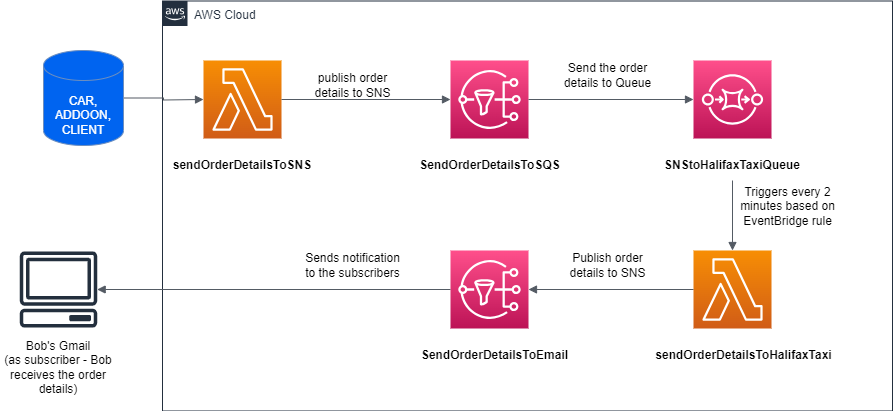
\includegraphics[scale=1, width=15cm]{PROBLEM 3/Screenshots/SDP-A3-Part C - Flowchart.png}
        \caption{\textbf{\textit{AWS Architecture diagram for the given work flow (Created using: draw.io [23])}}}
        \label{fig:aws-arch-diag}
    \end{figure}
% \newpage
\section{Steps}
\begin{enumerate}
    \item Create an IAM role with permissions to be : { invoked, publish messages to SNS, push messages to SQS } and attach to the lambda functions.
    \item Create a JSON file: \textbf{AssumeRolePolicyDocument.json} with the following contents (IAM role creation) [24]
    % Define custom colors for syntax highlighting
\definecolor{keyword}{RGB}{0, 0, 255}      % Blue for keywords
\definecolor{string}{RGB}{163, 21, 21}    % Red for strings
\definecolor{comment}{RGB}{0, 128, 0}     % Green for comments

% JSON language definition for listings package
\lstdefinelanguage{json}{
  basicstyle=\ttfamily\small,
  keywordstyle=\color{keyword}\bfseries,
  commentstyle=\color{comment}\itshape,
  stringstyle=\color{string},
  morecomment=[l]{//},
  morecomment=[s]{/*}{*/},
  moredelim=[is][\color{blue}\bfseries]{\{}{\}},
  moredelim=[is][\color{blue}\bfseries]{[}{]},
  identifierstyle=\color{blue}\bfseries,
  showstringspaces=false,
  breaklines=true
}


\begin{mdframed}[linewidth=1pt]
\lstset{language=json}
\begin{lstlisting}
{
{
    "Version": "2012-10-17",
    "Statement": [
        {
            "Effect": "Allow",
            "Principal": {
                "Service": "lambda.amazonaws.com"
            },
            "Action": "sts:AssumeRole"
        }
    ]
}
\end{lstlisting}
\end{mdframed}

    \item  Create another JSON file: \textbf{invokeFunction.json} with the following contents (add invokeFunction permission)
    % Define custom colors for syntax highlighting
\definecolor{keyword}{RGB}{0, 0, 255}      % Blue for keywords
\definecolor{string}{RGB}{163, 21, 21}    % Red for strings
\definecolor{comment}{RGB}{0, 128, 0}     % Green for comments

% JSON language definition for listings package
\lstdefinelanguage{json}{
  basicstyle=\ttfamily\small,
  keywordstyle=\color{keyword}\bfseries,
  commentstyle=\color{comment}\itshape,
  stringstyle=\color{string},
  morecomment=[l]{//},
  morecomment=[s]{/*}{*/},
  moredelim=[is][\color{blue}\bfseries]{\{}{\}},
  moredelim=[is][\color{blue}\bfseries]{[}{]},
  identifierstyle=\color{blue}\bfseries,
  showstringspaces=false,
  breaklines=true
}


\begin{mdframed}[linewidth=1pt]
\lstset{language=json}
\begin{lstlisting}
{
{
    "Version": "2012-10-17",
    "Statement": [
      {
        "Effect": "Allow",
        "Action": "lambda:InvokeFunction",
        "Resource": "*"
      }
    ]
}
\end{lstlisting}
\end{mdframed}

 \item Now, run the following commands to create the IAM role: \textbf{lambdaRole-Part-C} \textbf{specifying the path} to the above-created json file using \textbf{file://\textless /path/to/file_name\textgreater.json} [6]

% Define custom colors for syntax highlighting
\definecolor{keyword}{RGB}{0, 0, 255}      % Blue for keywords
\definecolor{string}{RGB}{163, 21, 21}    % Red for strings
\definecolor{comment}{RGB}{0, 128, 0}     % Green for comments

% PowerShell language definition for listings package
\lstdefinelanguage{PowerShell}{
  keywords={aws, lambda, add-permission, --function-name, --action, --principal, --source-arn, --statement-id},
  keywordstyle=\color{keyword}\bfseries,
  sensitive=false,
  morestring=[b]',
  morestring=[b]",
}


\begin{mdframed}[linewidth=1pt]
\lstset{language=PowerShell}
\begin{lstlisting}[basicstyle=\ttfamily\small, breaklines=true]
aws iam create-role --role-name lambdaRole-Part-C --assume-role-policy-document file://AssumeRolePolicyDocument.json

aws iam put-role-policy --role-name lambdaRole-Part-C --policy-name LambdaExecutionPolicy --policy-document file://invokeFunction.json
\end{lstlisting}
\end{mdframed}
   

    \item Run the following commands to add the permissions to the created lambda role \textbf{lambdaRole-Part-C} [25]
    
 % Define custom colors for syntax highlighting
\definecolor{keyword}{RGB}{0, 0, 255}      % Blue for keywords
\definecolor{string}{RGB}{163, 21, 21}    % Red for strings
\definecolor{comment}{RGB}{0, 128, 0}     % Green for comments

\lstdefinelanguage{AWSCLI}{
  keywords={aws, iam, attach-role-policy, --role-name, --policy-arn},
  keywordstyle=\color{keyword}\bfseries,
  sensitive=false,
  morestring=[b]',
  morestring=[b]",
}

\begin{mdframed}[linewidth=1pt]
\lstset{
  language=AWSCLI,
  basicstyle=\ttfamily\small,
  commentstyle=\color{comment}\itshape,
  breaklines=true,
}
\begin{lstlisting}
# AWSLambdaExecute role with permissions - Put, Get access to S3 and full access to CloudWatch Logs.
aws iam attach-role-policy --role-name lambdaRole-Part-C --policy-arn arn:aws:iam::aws:policy/AWSLambdaExecute

# AmazonSNSFullAccess role with permissions - Full access to SNS
aws iam attach-role-policy --role-name lambdaRole-Part-C --policy-arn arn:aws:iam::aws:policy/AmazonSNSFullAccess

# AmazonSQSFullAccess role with permissions - Full access to SQS
aws iam attach-role-policy --role-name lambdaRole-Part-C --policy-arn arn:aws:iam::aws:policy/AmazonSQSFullAccess
\end{lstlisting}
\end{mdframed}

    \item Run the following command to create a serverless-framework project [3]
    % Define custom colors for syntax highlighting
\definecolor{keyword}{RGB}{0, 0, 255}      % Blue for keywords
\definecolor{string}{RGB}{163, 21, 21}    % Red for strings
\definecolor{comment}{RGB}{0, 128, 0}     % Green for comments

\lstdefinelanguage{Serverless}{
  keywords={serverless, create, --template, aws-python3, --path},
  keywordstyle=\color{keyword}\bfseries,
  sensitive=false,
  morestring=[b]',
  morestring=[b]",
}


\begin{mdframed}[linewidth=1pt]
\lstset{
  language=Serverless,
  basicstyle=\ttfamily\small,
  commentstyle=\color{comment}\itshape,
  breaklines=true,
}
\begin{lstlisting}
# Create a new AWS Python3 Serverless project at path 'CarService'.
serverless create --template aws-python3 --path CarService
\end{lstlisting}
\end{mdframed}


\item Create the required resources using the following serverless framework script[3] (serverless.yml)[4] 


% Define custom colors for syntax highlighting
\definecolor{keyword}{RGB}{0, 0, 255}      % Blue for keywords
\definecolor{string}{RGB}{163, 21, 21}    % Red for strings
\definecolor{comment}{RGB}{0, 128, 0}     % Green for comments

% YAML language definition for listings package
\lstdefinelanguage{YAML}{
  keywords={service, provider, resources, Type, Properties, FunctionName, Code, Handler, Runtime, MemorySize, Timeout, Role, TableName, AttributeName, AttributeType, KeySchema, ProvisionedThroughput},
  keywordstyle=\color{keyword}\bfseries,
  sensitive=false,
  comment=[l]{\#},
  commentstyle=\color{comment}\ttfamily,
  stringstyle=\color{string}\ttfamily,
  morestring=[b]',
  morestring=[b]"
}


\begin{mdframed}[linewidth=1pt]
\lstset{language=YAML}
\begin{lstlisting}[basicstyle=\ttfamily\small, breaklines=true]
service: CarService
provider:
  name: aws
  runtime: python3.8
  region: us-east-1  
  stage: dev 

resources:
  Resources:
    # 1st Lambda Function to Send order details to SNS 
    SendOrderDetailsToSNS:
      Type: AWS::Lambda::Function
      Properties:
        FunctionName: sendOrderDetailsToSNS
        Code:
          ZipFile: | 
            import json
            def lambda_handler(event, context):
                # TODO implement
                return {
                    'statusCode': 200,
                    'body': json.dumps('Hello from Lambda!')
                }
        Handler: app.lambda_handler  # Ensure that the handler function name matches the code
        Runtime: python3.8
        MemorySize: 512
        Timeout: 10
        Role: arn:aws:iam::000966082997:role/lambdaRole-Part-C

    # 2nd Lambda Function to Send Order Details to Halifax Taxi
    SendOrderDetailsToHalifaxTaxi:
      Type: AWS::Lambda::Function
      Properties:
        FunctionName: sendOrderDetailsToHalifaxTaxi
        Code:
          ZipFile: |
            import json
            def lambda_handler(event, context):
                # TODO implement
                return {
                    'statusCode': 200,
                    'body': json.dumps('Hello from Lambda!')
                }
        Handler: app.handler  # Ensure that the handler function name matches the code
        Runtime: python3.8
        MemorySize: 512
        Timeout: 10
        Role: arn:aws:iam::000966082997:role/lambdaRole-Part-C

    # 1st SNS Topic - To take order details from Lambda and send to SQS
    SnsTopicToSqs:
      Type: AWS::SNS::Topic
      Properties:
        TopicName: SendOrderDetailsToSQS

    # 1st SNS Topic Subscription - Lambda subscribing to the SNS topic
    SnsSubscriptionToSqs:
      Type: AWS::SNS::Subscription
      Properties:
        TopicArn: !Ref SnsTopicToSqs
        Protocol: lambda
        Endpoint:
          Fn::GetAtt:
            - SendOrderDetailsToSNS
            - Arn

    # 2nd SNS Topic - To poll order details from SQS and publish to email
    SnsTopicToEmail:
      Type: AWS::SNS::Topic
      Properties:
        TopicName: SendOrderDetailsToEmail
        Subscription:
          - Protocol: email
            Endpoint: vikramvenkatapathi@gmail.com

    # 2nd SNS Topic Subscription - Lambda subscribing to the SNS topic
    SnsSubscriptionToEmail:
      Type: AWS::SNS::Subscription
      Properties:
        TopicArn: !Ref SnsTopicToEmail
        Protocol: lambda
        Endpoint:
          Fn::GetAtt:
            - SendOrderDetailsToHalifaxTaxi
            - Arn
    SNStoHalifaxTaxiQueue:
      Type: AWS::SQS::Queue
      Properties:
        QueueName: SNStoHalifaxTaxiQueue

    # SQS Queue Subscription - Subscribe SQS to SNS topic
    SqsSubscriptionToSns:
      Type: AWS::SNS::Subscription
      Properties:
        TopicArn: !Ref SnsTopicToSqs
        Protocol: sqs
        Endpoint:
          Fn::GetAtt:
            - SNStoHalifaxTaxiQueue
            - Arn

    # CloudWatch Events Rule to trigger Lambda function periodically every 2 minutes
    SendOrderDetailsToHalifaxTaxiSchedule:
      Type: AWS::Events::Rule
      Properties:
        ScheduleExpression: rate(2 minutes)
        Targets:
          - Arn: arn:aws:lambda:us-east-1:000966082997:function:sendOrderDetailsToHalifaxTaxi
            Id: SendOrderDetailsToHalifaxTaxiScheduleTarget

\end{lstlisting}
\end{mdframed}

\item The above script does the following
\begin{enumerate}
    \item Create 2 - lambdas: SendOrderDetailsToSNS, SendOrderDetailsToHalifaxTaxi
    \item Create 2 - SNS topics: SendOrderDetailsToSQS, SendOrderDetailsToEmail
    \item Create 1 - SQS Queue: SNStoHalifaxTaxiQueue
    \item Create 2 subscriptions for SNS topic SendOrderDetailsToSQS
    \begin{enumerate}
        \item Lambda - SendOrderDetailsToSNS
        \item SQS - SNStoHalifaxTaxiQueue
    \end{enumerate}
    \item Create 2 subscriptions for SNS topic SendOrderDetailsToEmail
    \begin{enumerate}
        \item Lambda - sendOrderDetailsToHalifaxTaxi
        \item Bob's Email - vikramvenkatapathi@gmail.com (my personal email)
    \end{enumerate}
    \item Create a CloudWatch Events Rule - SendOrderDetailsToHalifaxTaxiSchedule, to trigger Lambda function: sendOrderDetailsToHalifaxTaxi, periodically every 2 minutes.

\end{enumerate}
\item Run the command \textbf{serverless deploy} to deploy the .yml file to create the resources in CloudFormation.

\section{Lambda Code}
\subsection{sendOrderDetailsToSNS}
% Define custom colors for syntax highlighting
\definecolor{keyword}{RGB}{0, 0, 255}      % Blue for keywords
\definecolor{string}{RGB}{163, 21, 21}    % Red for strings
\definecolor{comment}{RGB}{0, 128, 0}     % Green for comments

\lstdefinestyle{mystyle}{
    basicstyle=\ttfamily\small,
    keywordstyle=\color{keyword}\bfseries,
    commentstyle=\color{comment}\itshape,
    stringstyle=\color{string},
    showstringspaces=false,
    breaklines=true
}


\begin{mdframed}[linewidth=1pt]
\lstset{style=mystyle}
\begin{lstlisting}[language=Python]
import json
import boto3
import random

# Sample data lists
car_types = ["Compact", "Mid-size Sedan", "SUV", "Luxury"]
car_accessories = ["GPS", "Camera", "Sun shades", "Vehicle Seat Cover"]
client_addresses = ["123 Main St", "456 Elm St", "789 Oak St", "1333 South park st"]

def lambda_handler(event, context):

    """
        W3schools - Python Random Module Documentation
        Reference: `W3schools - Python Random Module <https://www.w3schools.com/python/module_random.asp>`_
    """
    # Generate a single message by combining data from all three lists
    order_details = {
        "type": "ORDER",
        "data": {
            "CAR_TYPE": random.choice(car_types),
            "CAR_ACCESSORY": random.choice(car_accessories),
            "CLIENT_ADDRESS": random.choice(client_addresses)
        }
    }

    # Publish the combined message to the SNS topic
    sns_topic_arn = "arn:aws:sns:us-east-1:000966082997:SendOrderDetailsToSQS"
    publish_to_sns(sns_topic_arn, order_details)
    
    print(order_details)
    return {
        'statusCode': 200,
        'body': json.dumps('Message sent to SNS topic=SendOrderDetailsToSQS!')
    }

def publish_to_sns(topic_arn, message):

    """
        Boto3 - Amazon Amazon Simple Notification Service (SNS) Documentation
        Reference: `Boto3 - Amazon SNS API <https://boto3.amazonaws.com/v1/documentation/api/latest/reference/services/sns.html>`_
    """
    sns_client = boto3.client('sns')

    sns_client.publish(
        TopicArn=topic_arn,
        Message=json.dumps(message)
    )

"""
All references:
    Boto3 - Amazon Amazon Simple Notification Service (SNS) Documentation
    Reference: `Boto3 - Amazon SNS API <https://boto3.amazonaws.com/v1/documentation/api/latest/reference/services/sns.html>`_

    W3schools - Python Random Module Documentation
    Reference: `W3schools - Python Random Module <https://www.w3schools.com/python/module_random.asp>`_
    
"""

\end{lstlisting}
\end{mdframed}
\subsection{sendOrderDetailsToHalifaxTaxi}
% Define custom colors for syntax highlighting
\definecolor{keyword}{RGB}{0, 0, 255}      % Blue for keywords
\definecolor{string}{RGB}{163, 21, 21}    % Red for strings
\definecolor{comment}{RGB}{0, 128, 0}     % Green for comments

\lstdefinestyle{mystyle}{
    basicstyle=\ttfamily\small,
    keywordstyle=\color{keyword}\bfseries,
    commentstyle=\color{comment}\itshape,
    stringstyle=\color{string},
    showstringspaces=false,
    breaklines=true
}


\begin{mdframed}[linewidth=1pt]
\lstset{style=mystyle}
\begin{lstlisting}[language=Python]
import json
import boto3

def handler(event, context):
    # Get the SQS queue URL
    queue_url = "https://sqs.us-east-1.amazonaws.com/000966082997/SNStoHalifaxTaxiQueue"

    """
        Boto3 - Amazon Amazon Simple Queue  Service (SQS) Documentation
        Reference: `Boto3 - Amazon SQS API <https://boto3.amazonaws.com/v1/documentation/api/latest/reference/services/sqs.html>`_
    """

    # Create an SQS client
    sqs = boto3.client('sqs')

    # Receive messages from the SQS queue (max 1 message)
    response = sqs.receive_message(
        QueueUrl=queue_url,
        MaxNumberOfMessages=1,
        VisibilityTimeout=30, 
        WaitTimeSeconds=0  # Set to 0 for non-blocking receive
    )

    # Check if any messages were received
    if 'Messages' in response:
        # Extract the message
        message = response['Messages'][0]
        body = json.loads(message['Body'])
        order_details = body['Message']
        # print(order_details)
        
        order_details_json = json.loads(order_details)
        
        # Template for the email body
        email_body_template = """Car Type : {car_type}, Car Accessory : {car_accessory}, Client Address : {client_address}"""

        """
            W3schools - Python String format() Method Documentation
            Reference: `W3schools - Python String format() Method <https://www.w3schools.com/python/ref_string_format.asp>`_
        """
        # Replace the placeholders in the email_body template
        email_body = email_body_template.format(
            car_type=order_details_json['data']['CAR_TYPE'],
            car_accessory=order_details_json['data']['CAR_ACCESSORY'],
            client_address=order_details_json['data']['CLIENT_ADDRESS']
        )

        # Publish the message to the SNS topic
        sns_topic_arn = "arn:aws:sns:us-east-1:000966082997:SendOrderDetailsToEmail"
        
        publish_to_sns(sns_topic_arn, email_body)

        # Delete the message from the SQS queue
        sqs.delete_message(
            QueueUrl=queue_url,
            ReceiptHandle=message['ReceiptHandle']
        )

    return {
        'statusCode': 200,
        'body': json.dumps('Message sent to subscriber')
    }

def publish_to_sns(topic_arn, message):
    # Create an SNS client
    sns = boto3.client('sns')

    """
        Boto3 - Amazon Amazon Simple Notification Service (SNS) Documentation
        Reference: `Boto3 - Amazon SNS API <https://boto3.amazonaws.com/v1/documentation/api/latest/reference/services/sns.html>`_
    """
    # Publish the message to the SNS topic
    sns.publish(
        TopicArn=topic_arn,
        Subject="Your order details",
        Message=json.dumps(message)
    )

"""
All references:
    Boto3 - Amazon Amazon Simple Notification Service (SNS) Documentation
    Reference: `Boto3 - Amazon SNS API <https://boto3.amazonaws.com/v1/documentation/api/latest/reference/services/sns.html>`_

    Boto3 - Amazon Amazon Simple Queue  Service (SQS) Documentation
    Reference: `Boto3 - Amazon SQS API <https://boto3.amazonaws.com/v1/documentation/api/latest/reference/services/sqs.html>`_

    W3schools - Python Random Module Documentation
    Reference: `W3schools - Python Random Module <https://www.w3schools.com/python/module_random.asp>`_
    
"""
\end{lstlisting}
\end{mdframed}
\section{Testing}
I followed the below testing procedure
\begin{enumerate}
    \item Triggered the 1st lambda \textbf{SendOrderDetailsToSNS} 2 times.
    \item Checked it logs - 2 messageBody's were present.
    \item Check if it published the messages to the SNS topic \textbf{SnsTopicToSqs}.
    \item Polled the messages in SQS \textbf{SNStoHalifaxTaxiQueue}, and verified that I received the 2 messages.
    \item Checked the logs of 2nd lambda \textbf{SendOrderDetailsToHalifaxTaxi}, and verified that messages are received periodically every 2 minutes based on the EventBridge rule.
    \item Verified the receipt of mail in Gmail.
\end{enumerate}

\end{enumerate}


\section{Screenshots}

    \begin{figure}[htp]
        \centering
        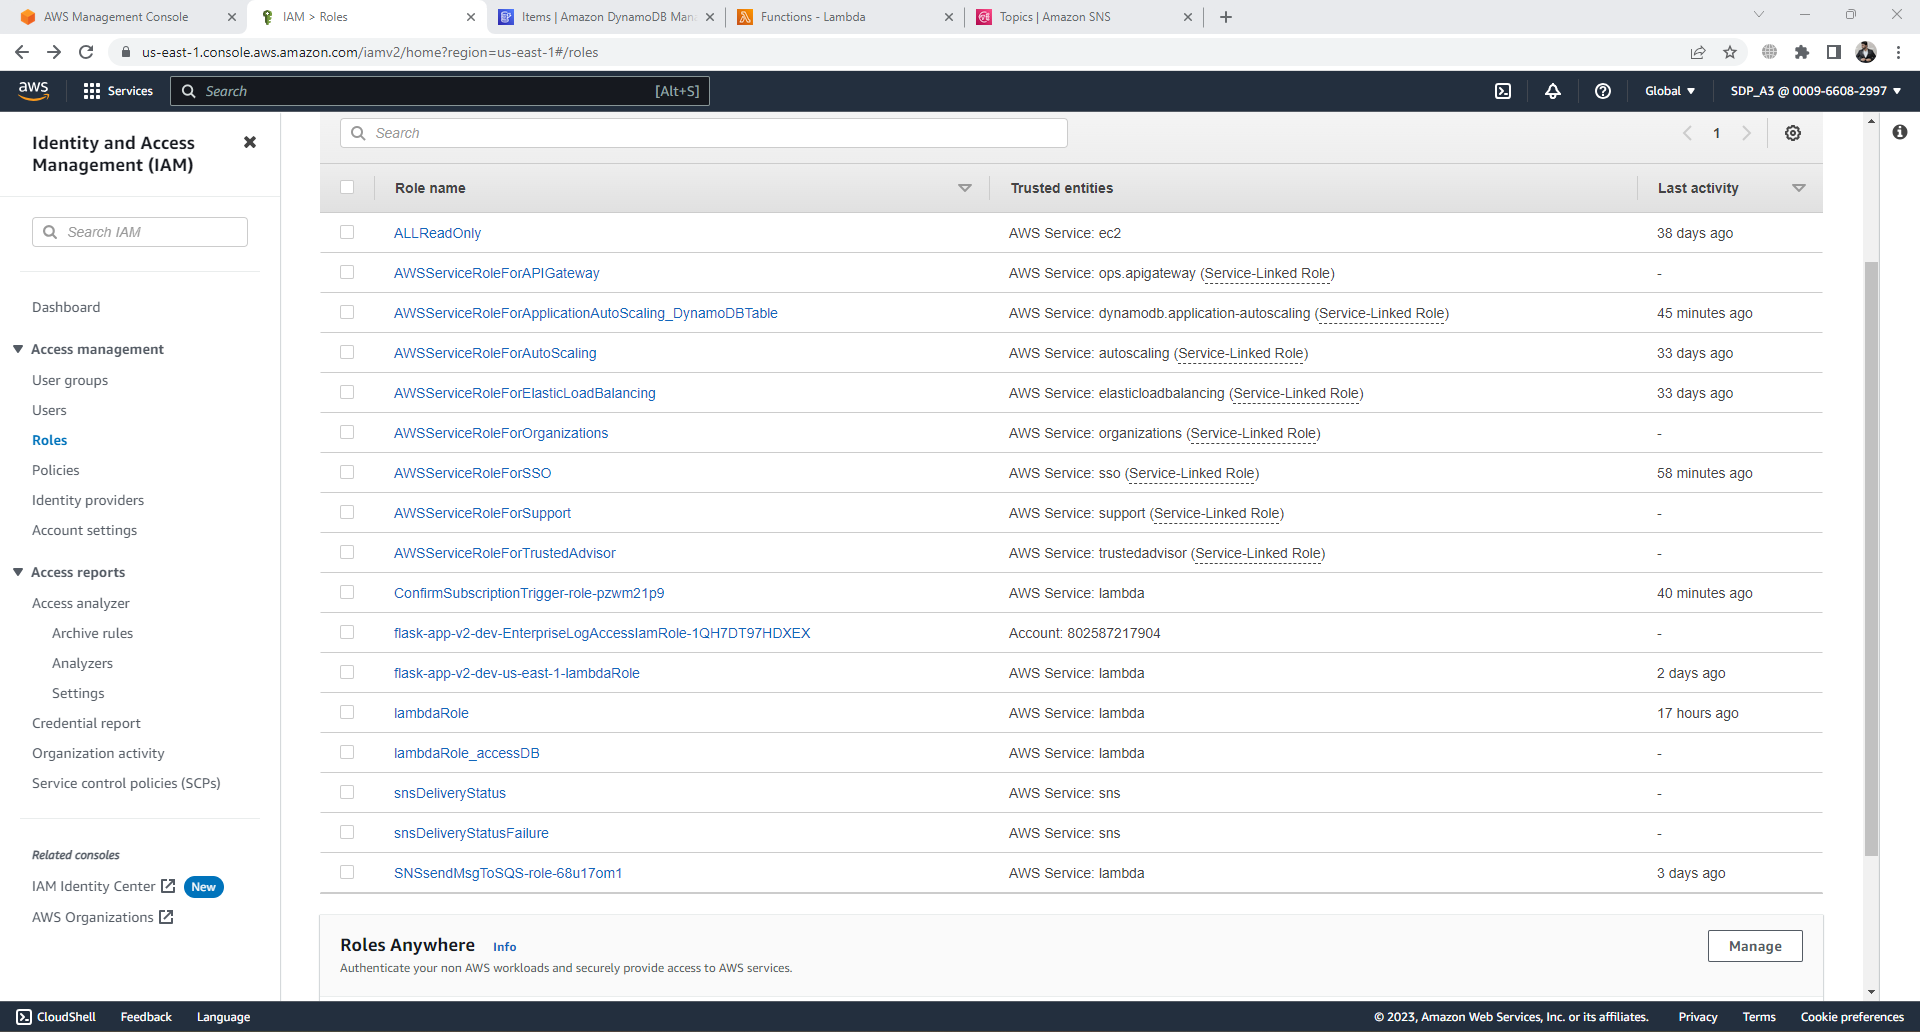
\includegraphics[scale=1, width=15cm]{PROBLEM 3/Screenshots/1. before role creation.png}
        \caption{\textbf{\textit{Before IAM Role creation}}}
        \label{fig:}
    \end{figure}

    \begin{figure}[htp]
        \centering
        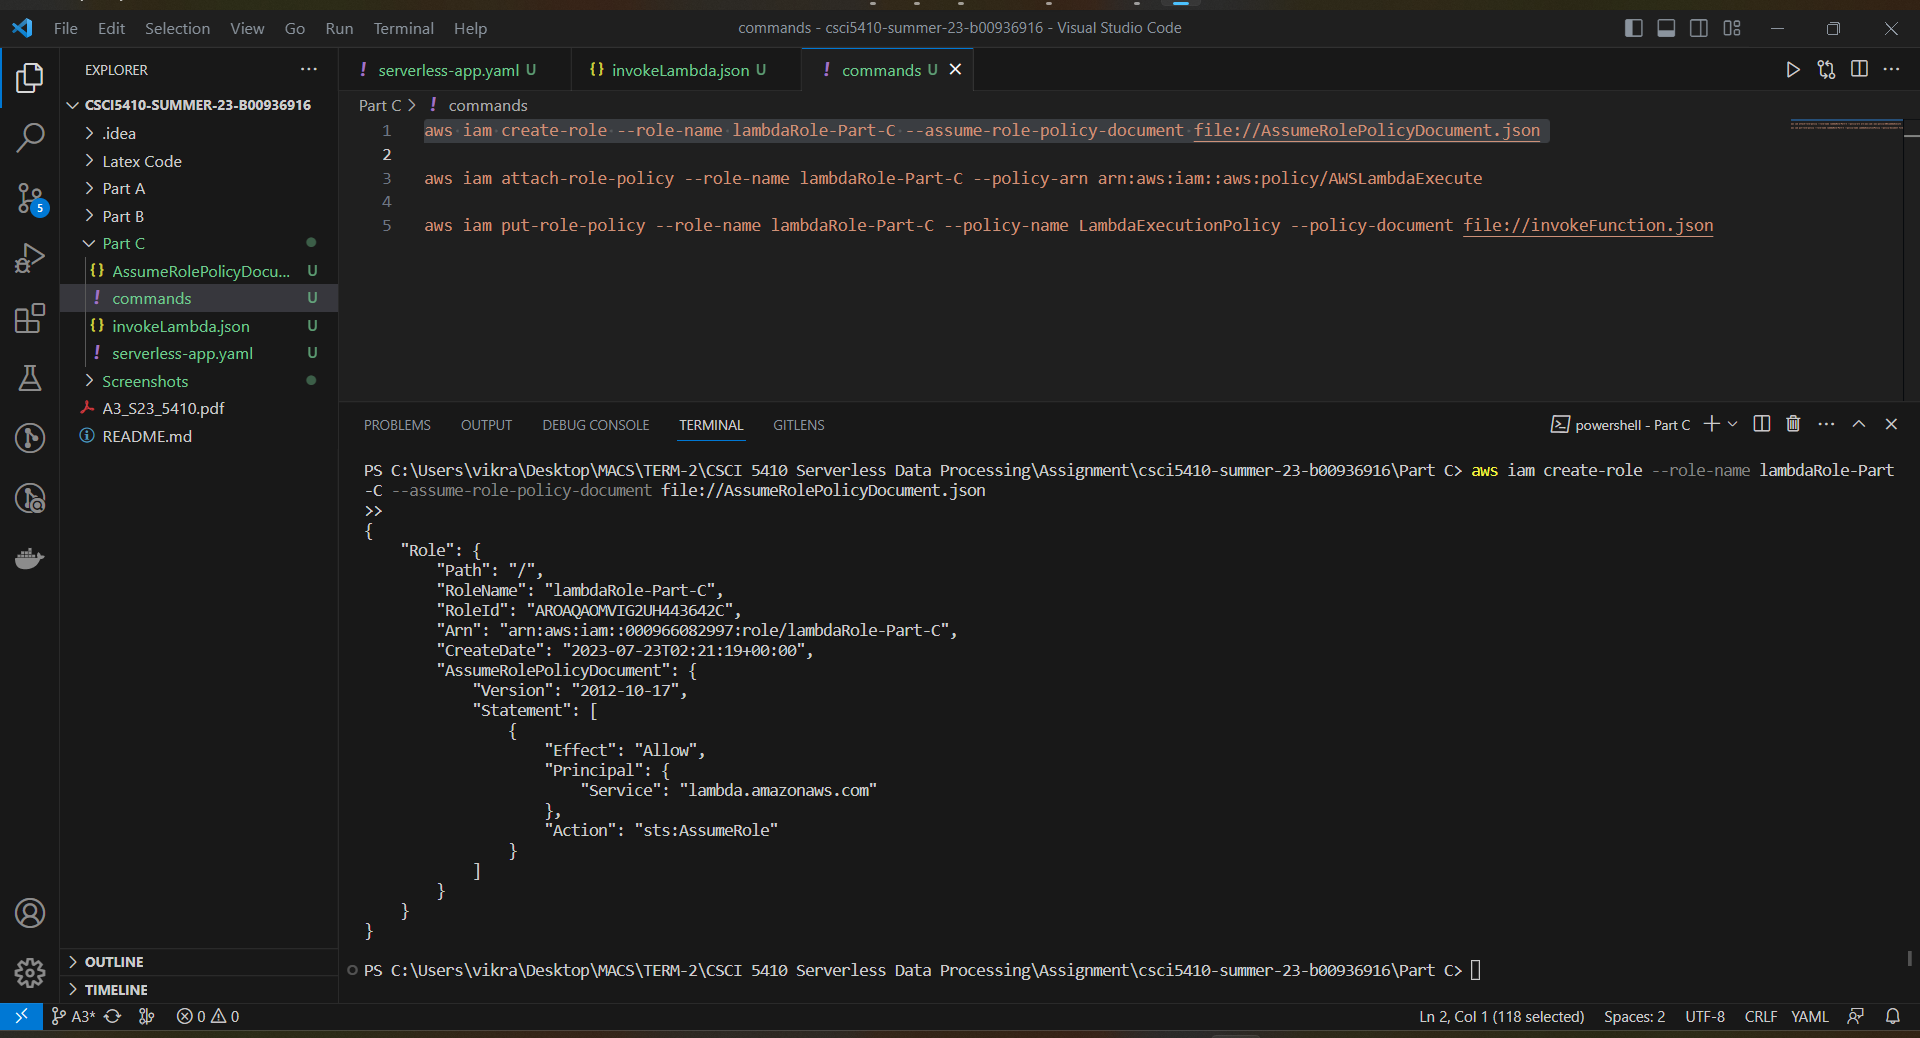
\includegraphics[scale=1, width=15cm]{PROBLEM 3/Screenshots/1.2 created role lambdaRole-Part-C in CLI.png}
        \caption{\textbf{\textit{Created IAM role lambdaRole-Part-C in CLI}}}
        \label{fig:}
    \end{figure}

     \begin{figure}[htp]
        \centering
        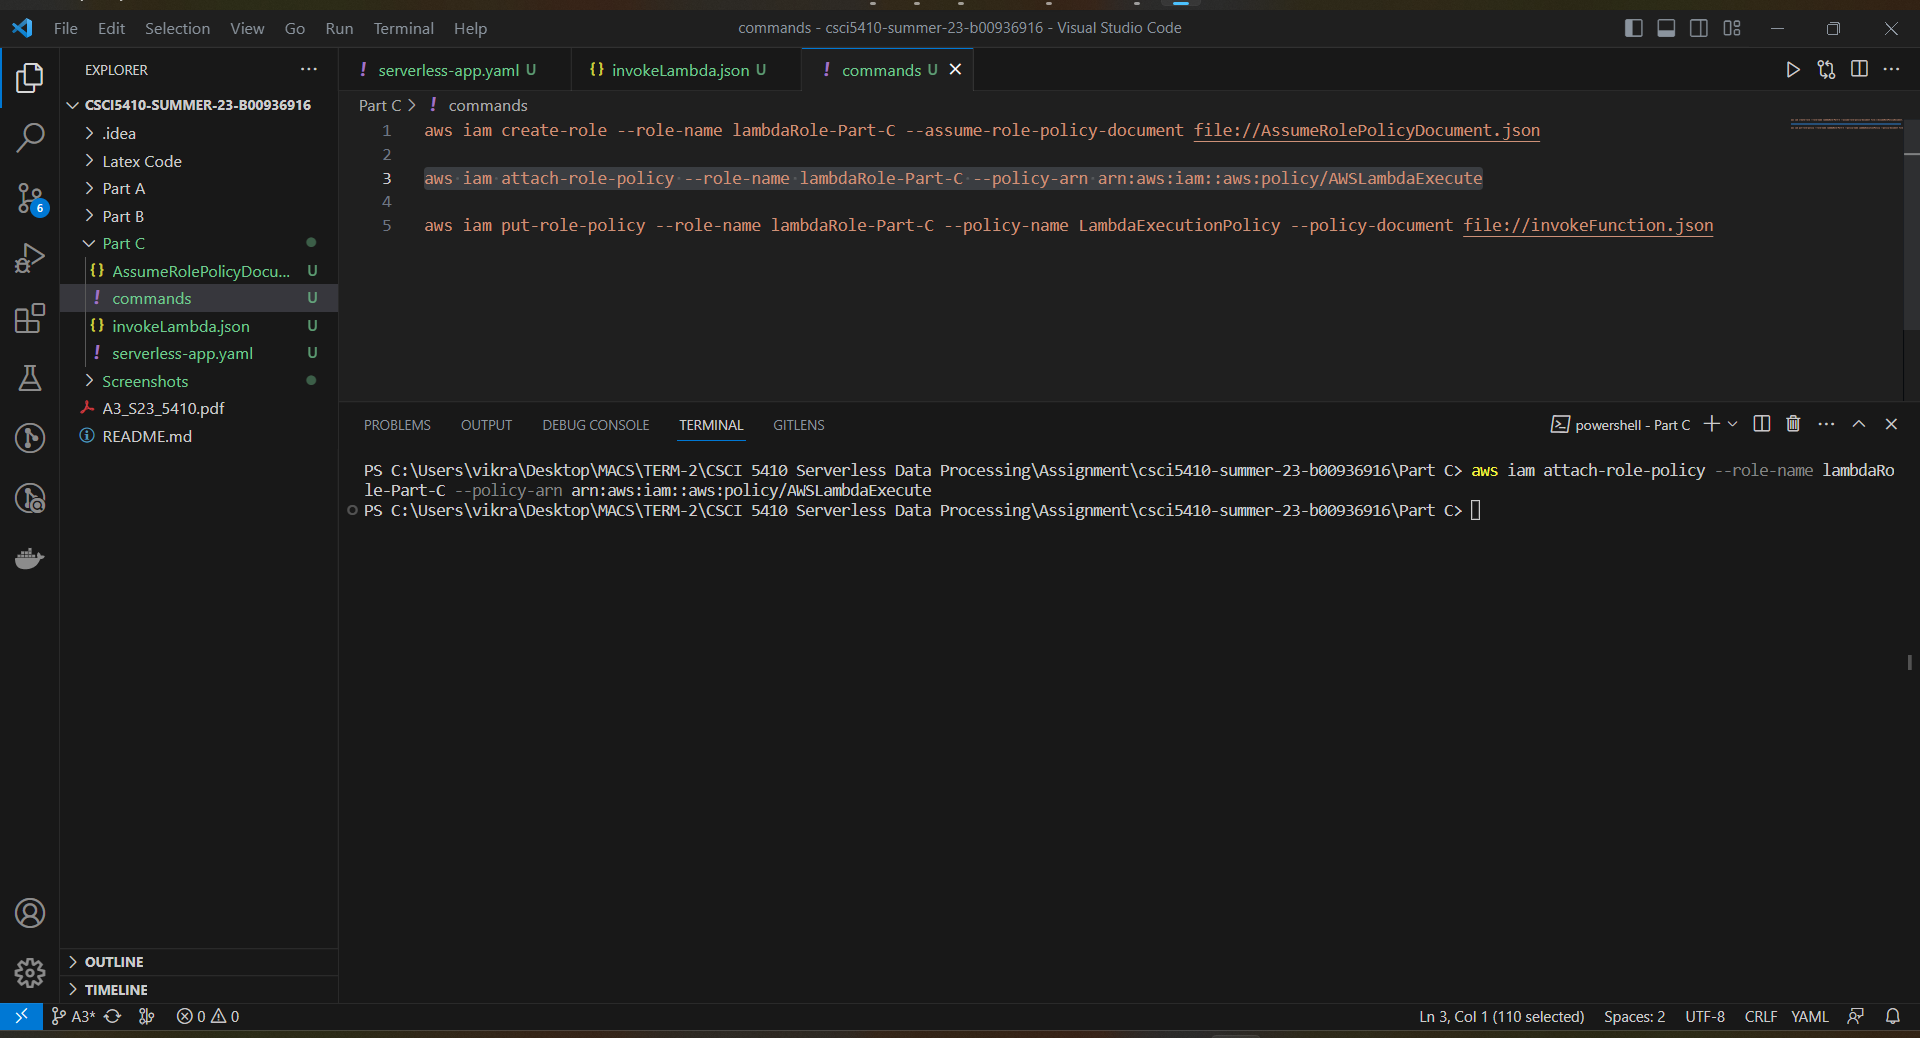
\includegraphics[scale=1, width=15cm]{PROBLEM 3/Screenshots/1.3 attach AWSLambdaExecute permission to role.png}
        \caption{\textbf{\textit{Attach AWSLambdaExecute permission to role: lambdaRole-Part-C}}}
        \label{fig:}
    \end{figure}

     \begin{figure}[htp]
        \centering
        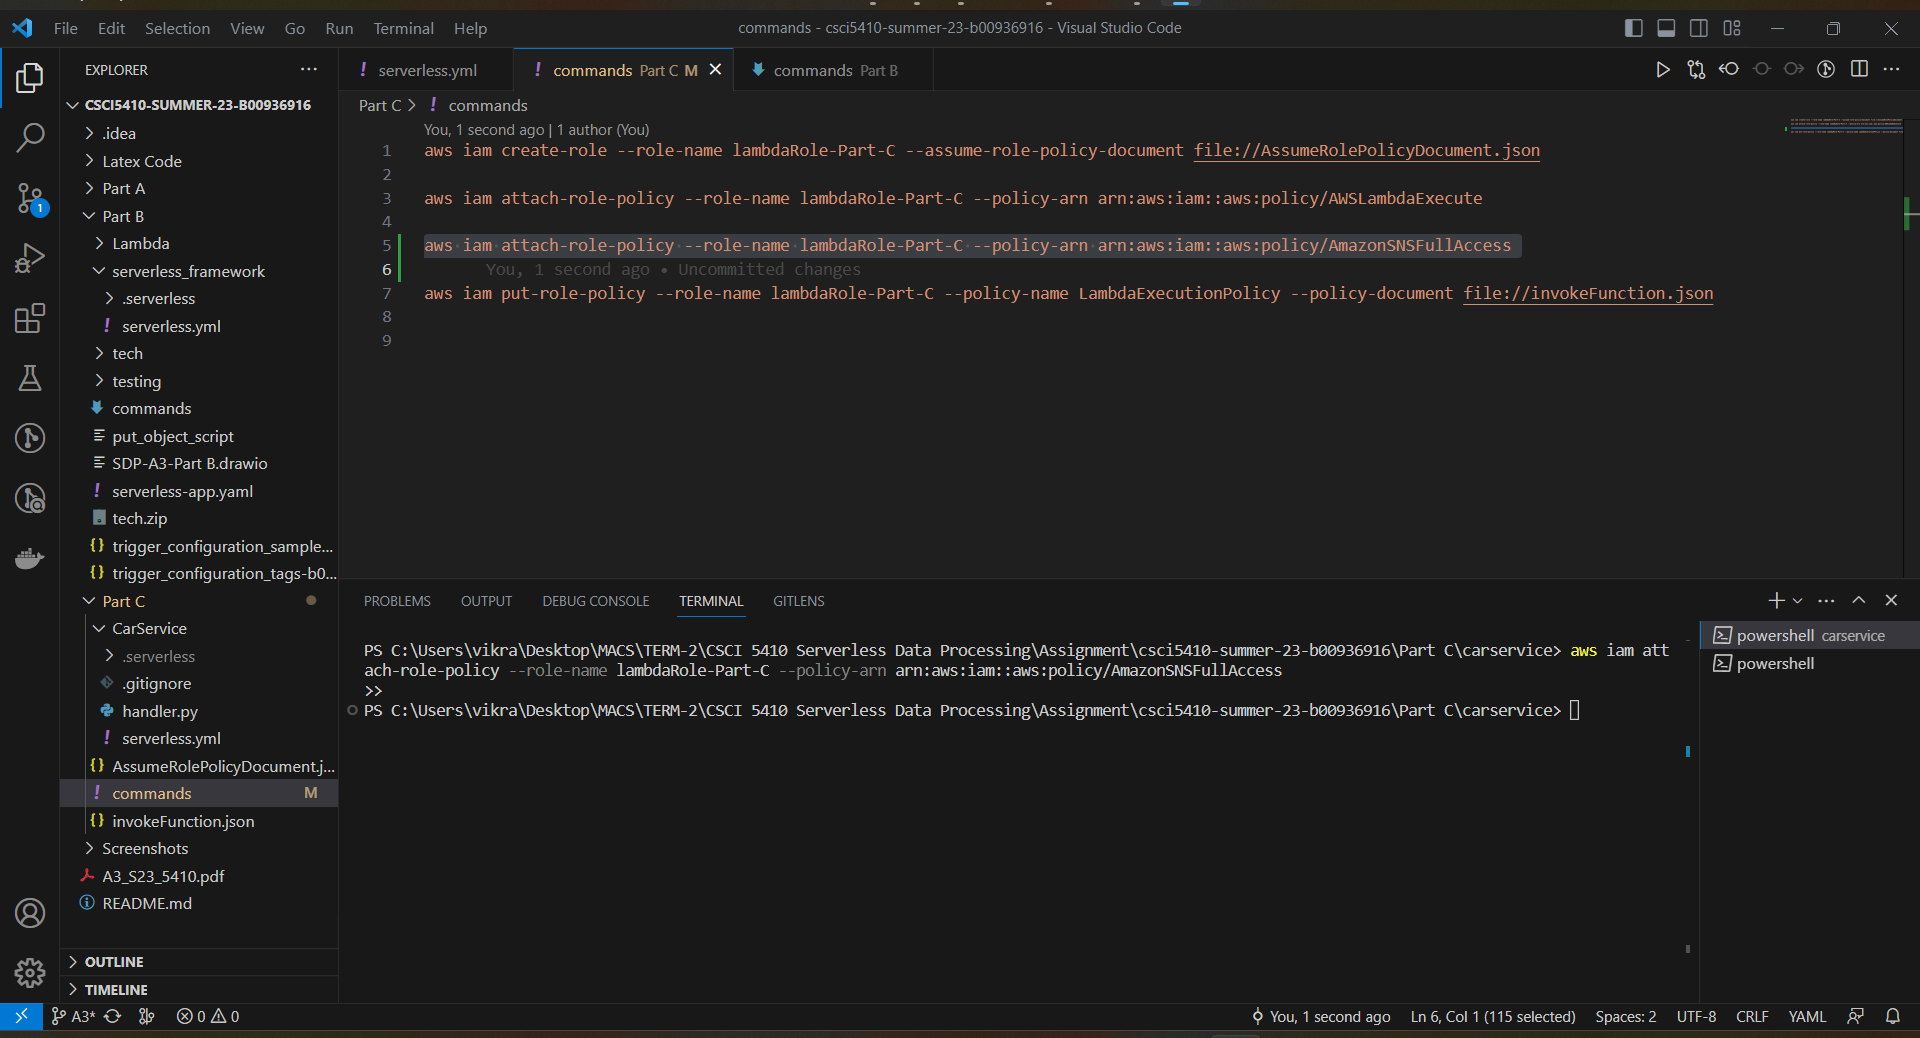
\includegraphics[scale=1, width=15cm]{PROBLEM 3/Screenshots/1.3.1 attach AmazonSNSFullAccess permission to role.png}
        \caption{\textbf{\textit{Attach AmazonSNSFullAccess permission to role: lambdaRole-Part-C}}}
        \label{fig:}
    \end{figure}


    \begin{figure}[htp]
        \centering
        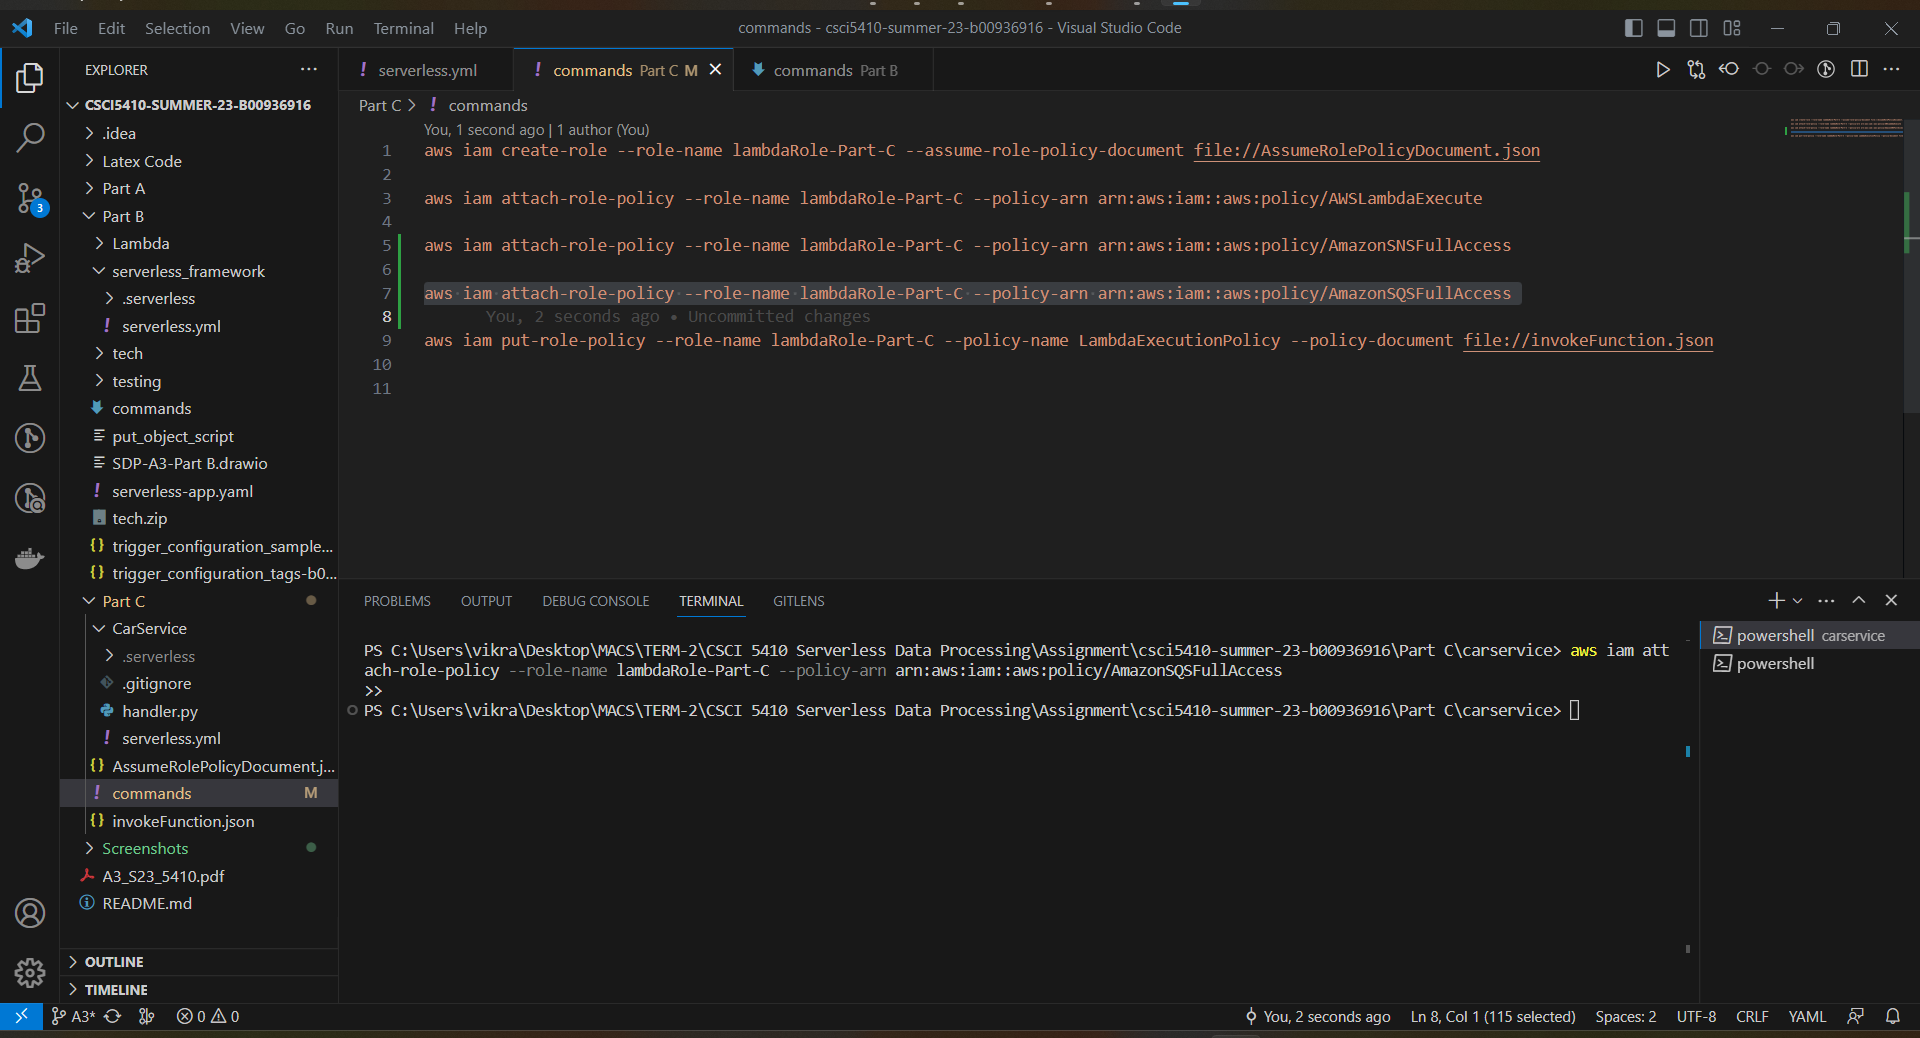
\includegraphics[scale=1, width=15cm]{PROBLEM 3/Screenshots/1.3.2 attach AmazonSQSFullAccess permission to role.png}
        \caption{\textbf{\textit{Attach AmazonSQSFullAccess permission to role: lambdaRole-Part-C}}}
        \label{fig:}
    \end{figure}

    \begin{figure}[htp]
        \centering
        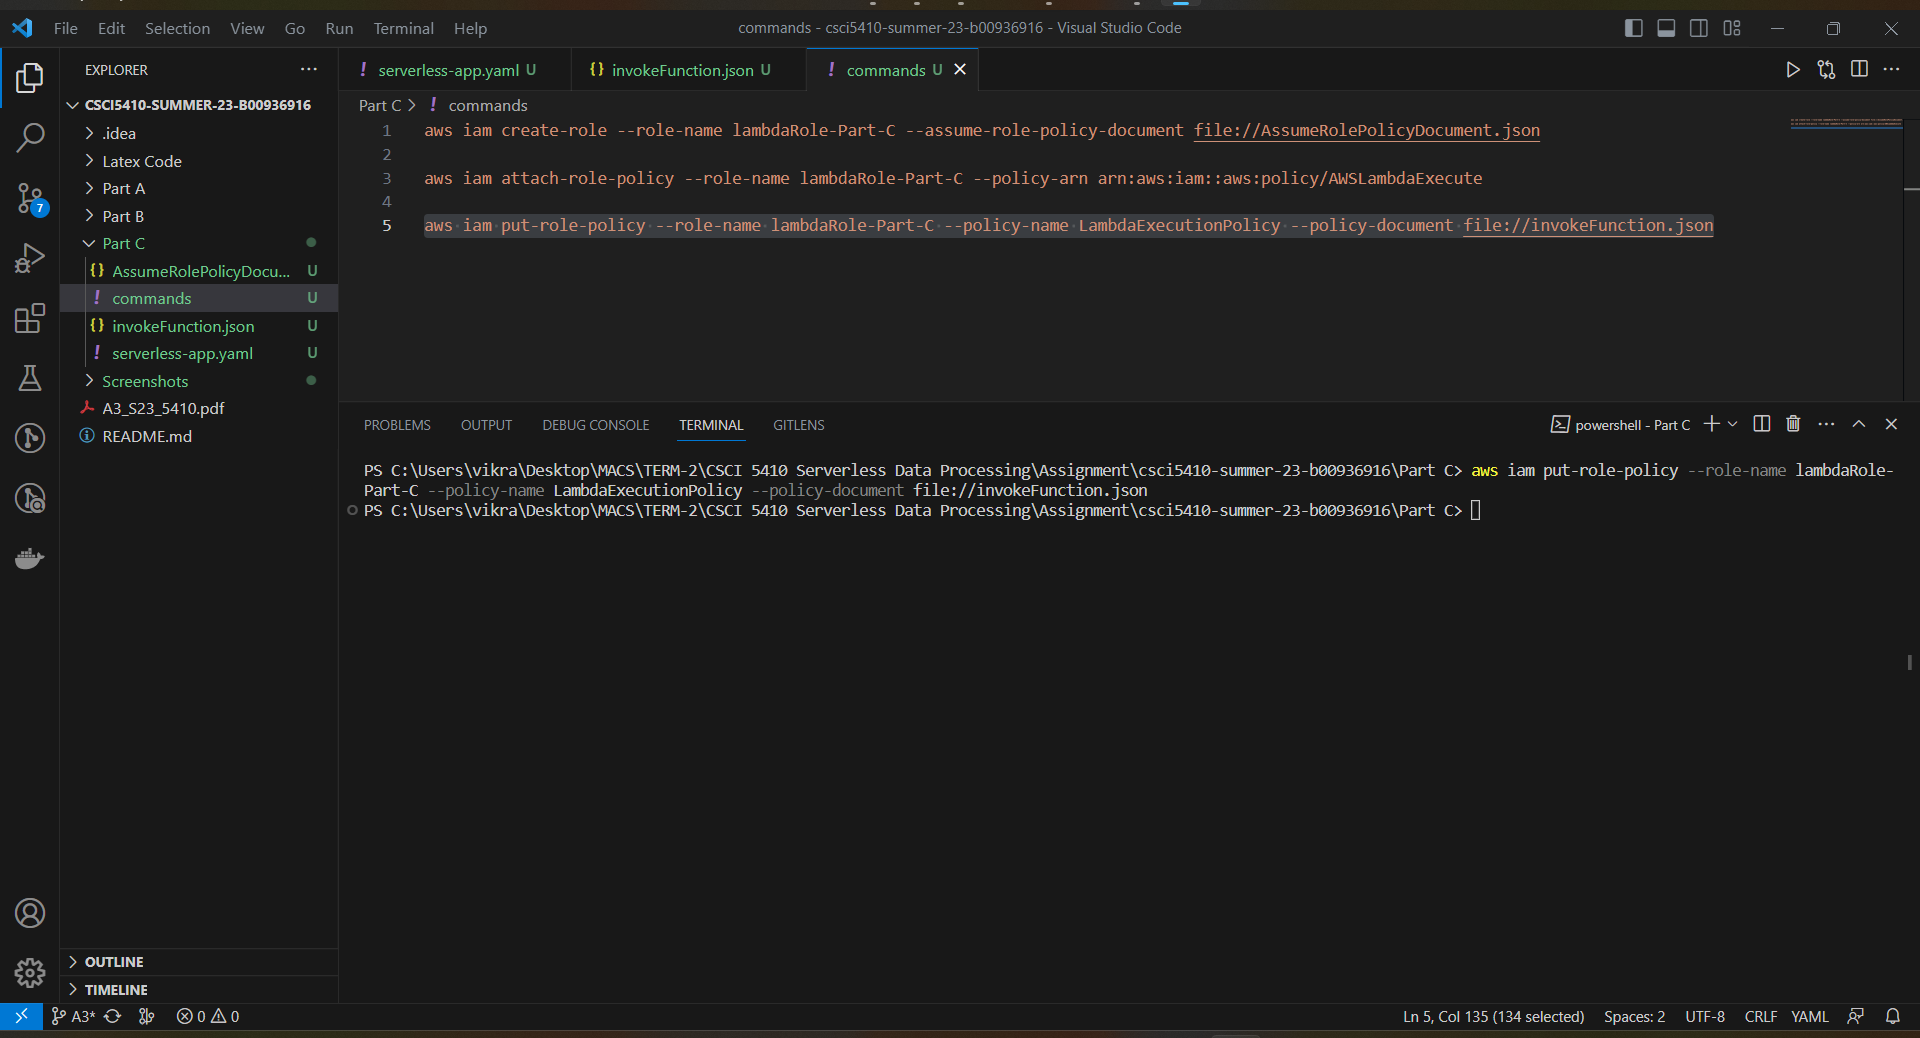
\includegraphics[scale=1, width=15cm]{PROBLEM 3/Screenshots/1.4 added invokeFunction permission.png}
        \caption{\textbf{\textit{Added invokeFunction permission to role: lambdaRole-Part-C}}}
        \label{fig:}
    \end{figure}

    \begin{figure}[htp]
        \centering
        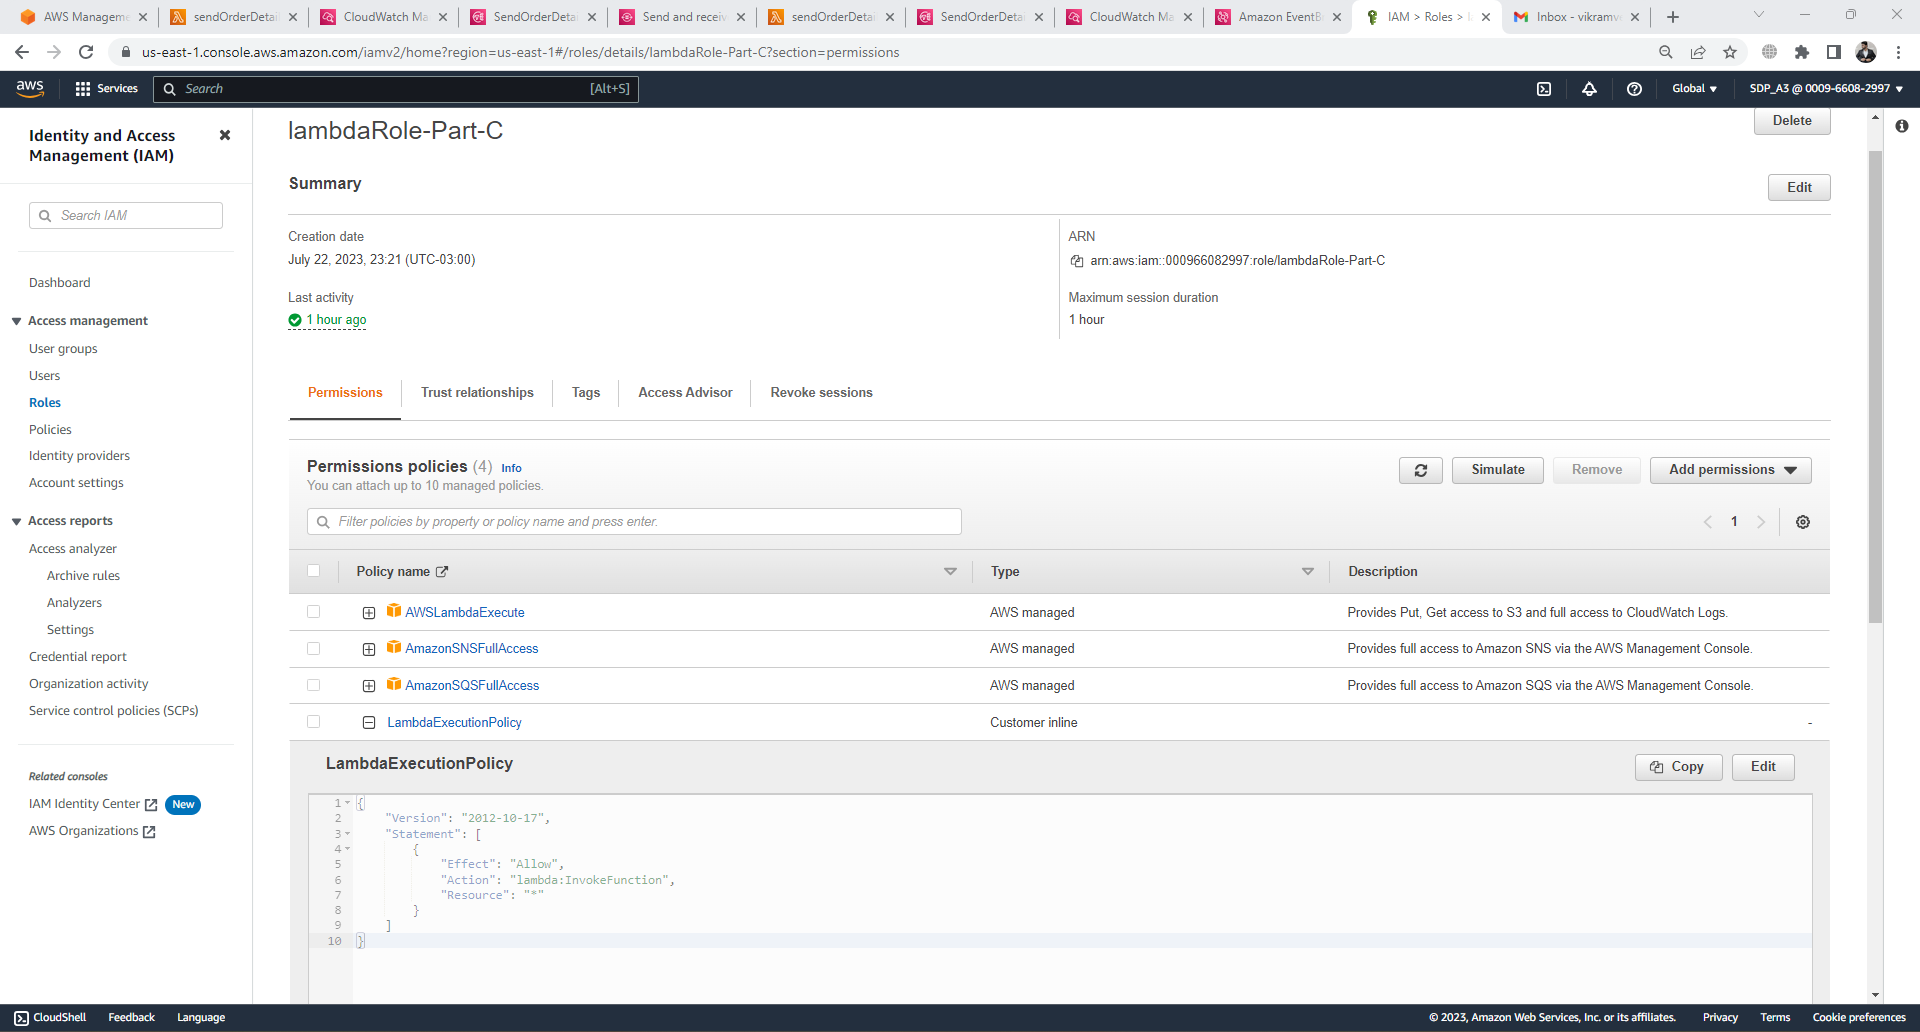
\includegraphics[scale=1, width=15cm]{PROBLEM 3/Screenshots/1.5 created permissions shown in console.png}
        \caption{\textbf{\textit{Created IAM role lambdaRole-Part-C's permissions shown in console}}}
        \label{fig:}
    \end{figure}

    \begin{figure}[htp]
        \centering
        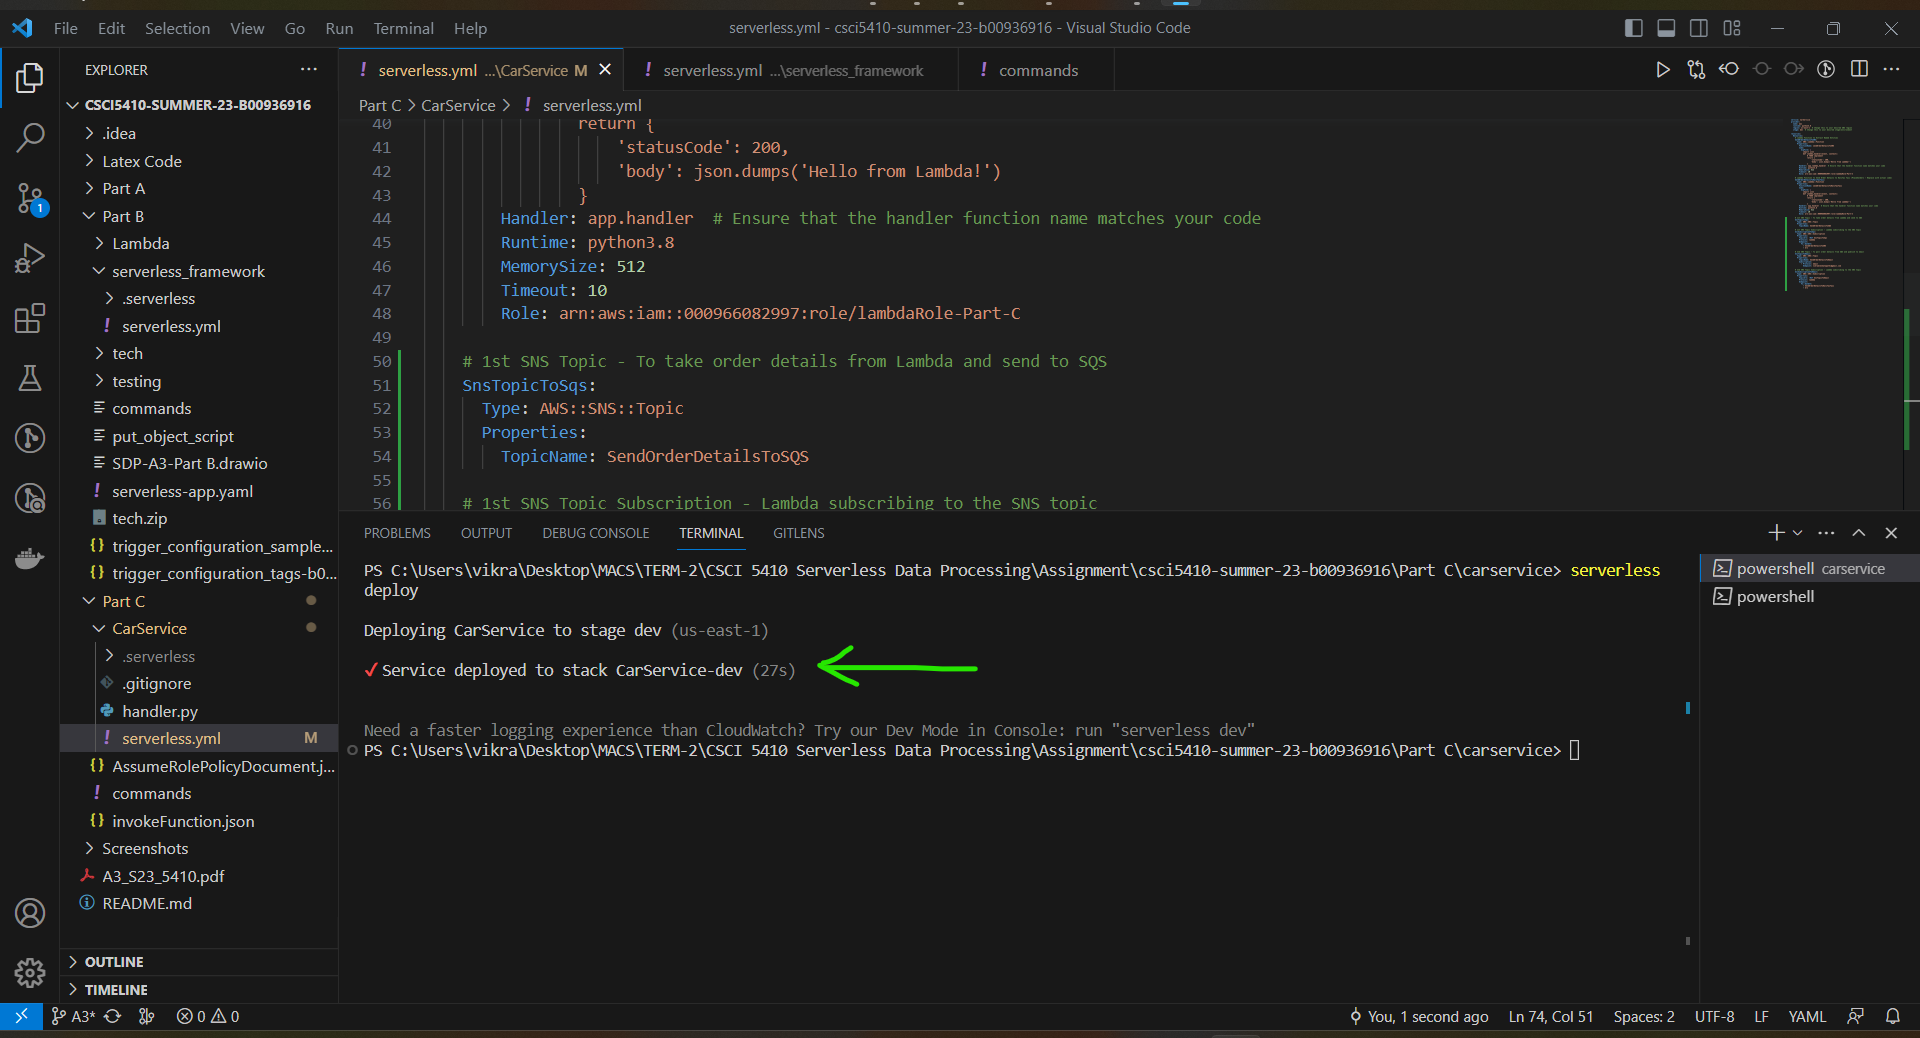
\includegraphics[scale=1, width=15cm]{PROBLEM 3/Screenshots/2.1 serverless.yml file executed in cli .png}
        \caption{\textbf{\textit{serverless.yml file executed in CLI }}}
        \label{fig:}
    \end{figure}

    \begin{figure}[htp]
        \centering
        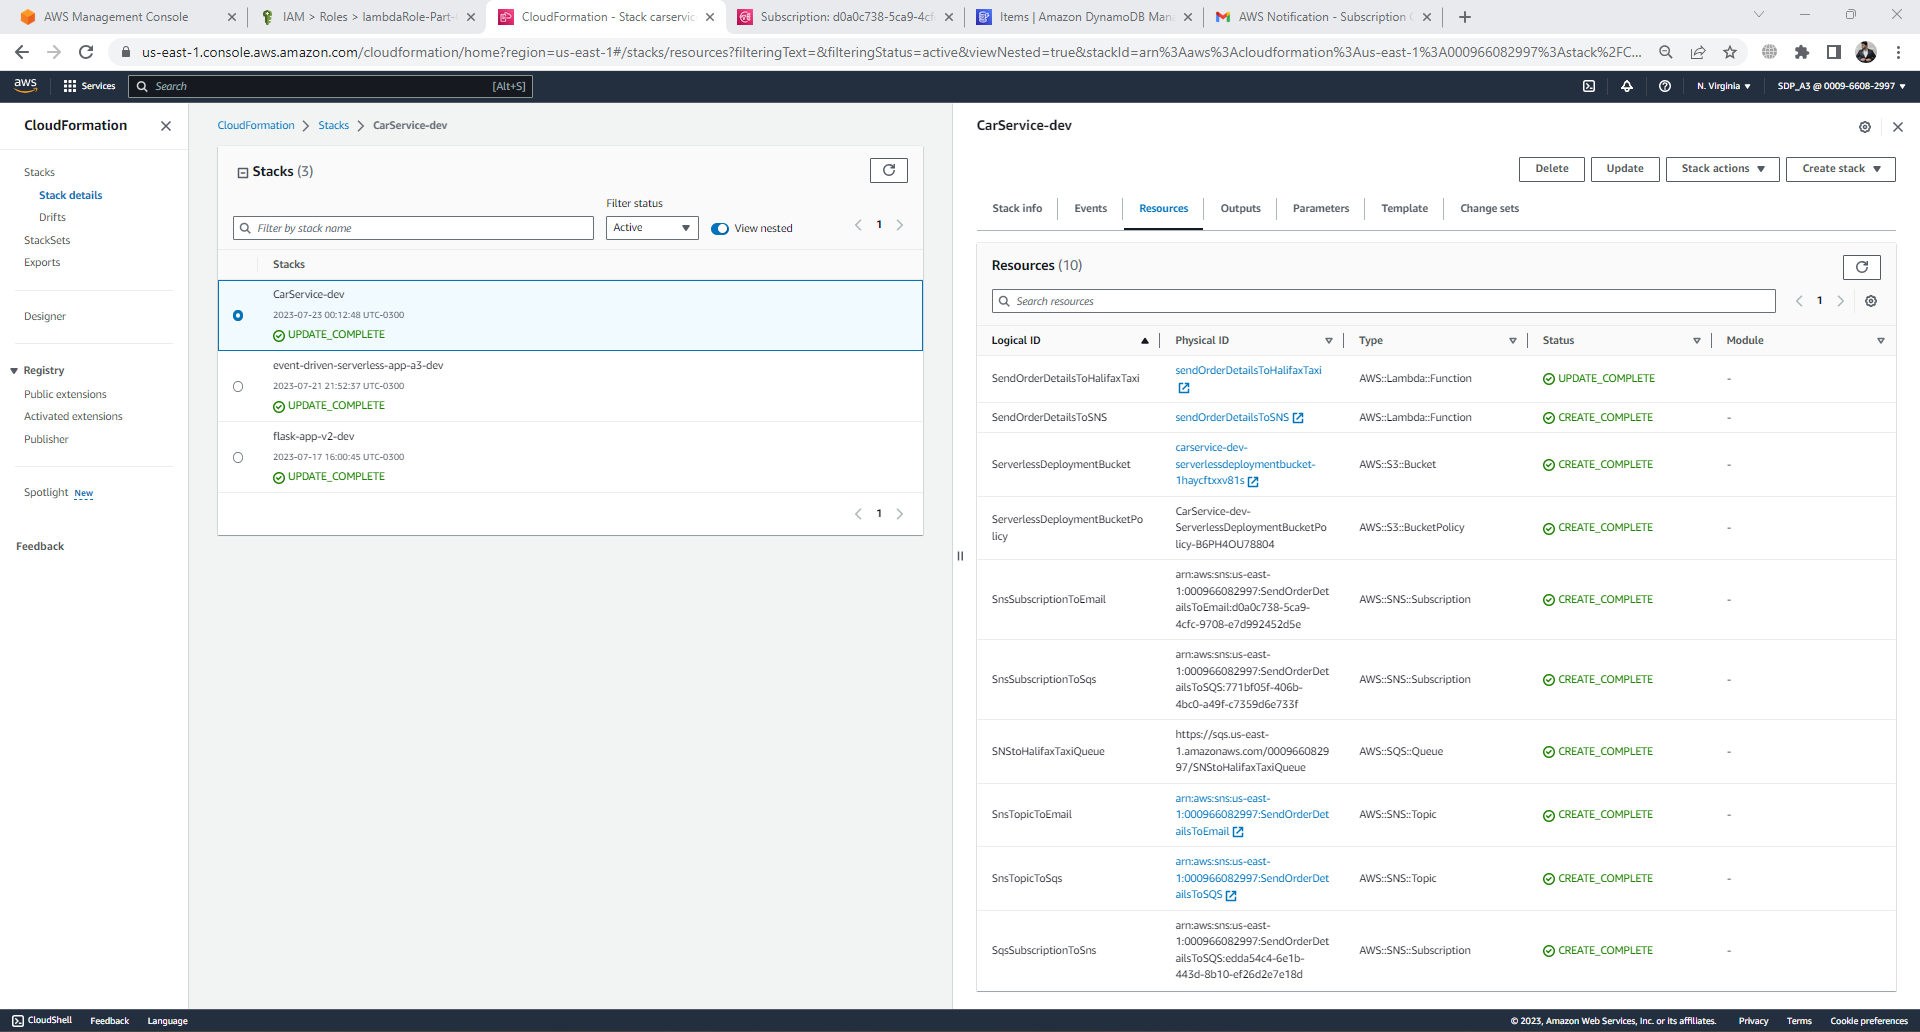
\includegraphics[scale=1, width=15cm]{PROBLEM 3/Screenshots/2.2 tech stacck created - shown in console.png}
        \caption{\textbf{\textit{Cloud formation stack created - shown in console}}}
        \label{fig:}
    \end{figure}

    \begin{figure}[htp]
        \centering
        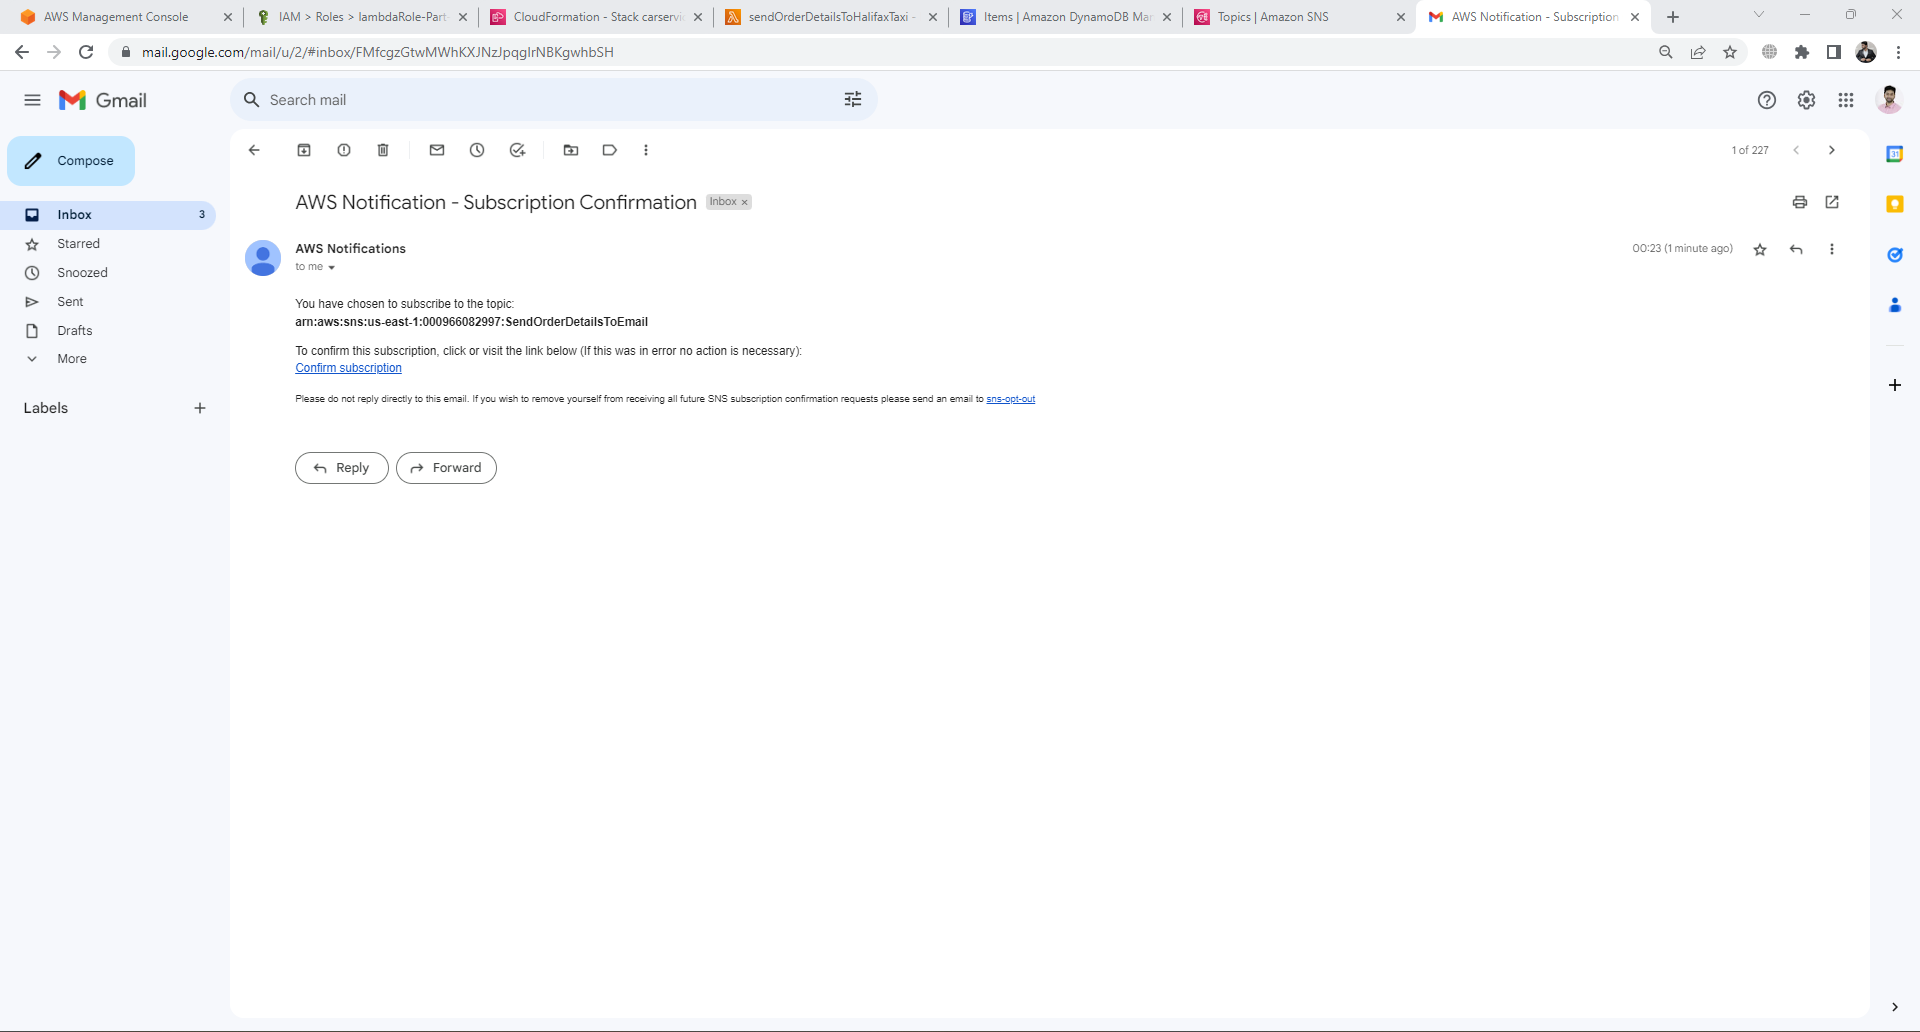
\includegraphics[scale=1, width=15cm]{PROBLEM 3/Screenshots/2.3 subsctription mail received.png}
        \caption{\textbf{\textit{Subscription mail received}}}
        \label{fig:}
    \end{figure}

    \begin{figure}[htp]
        \centering
        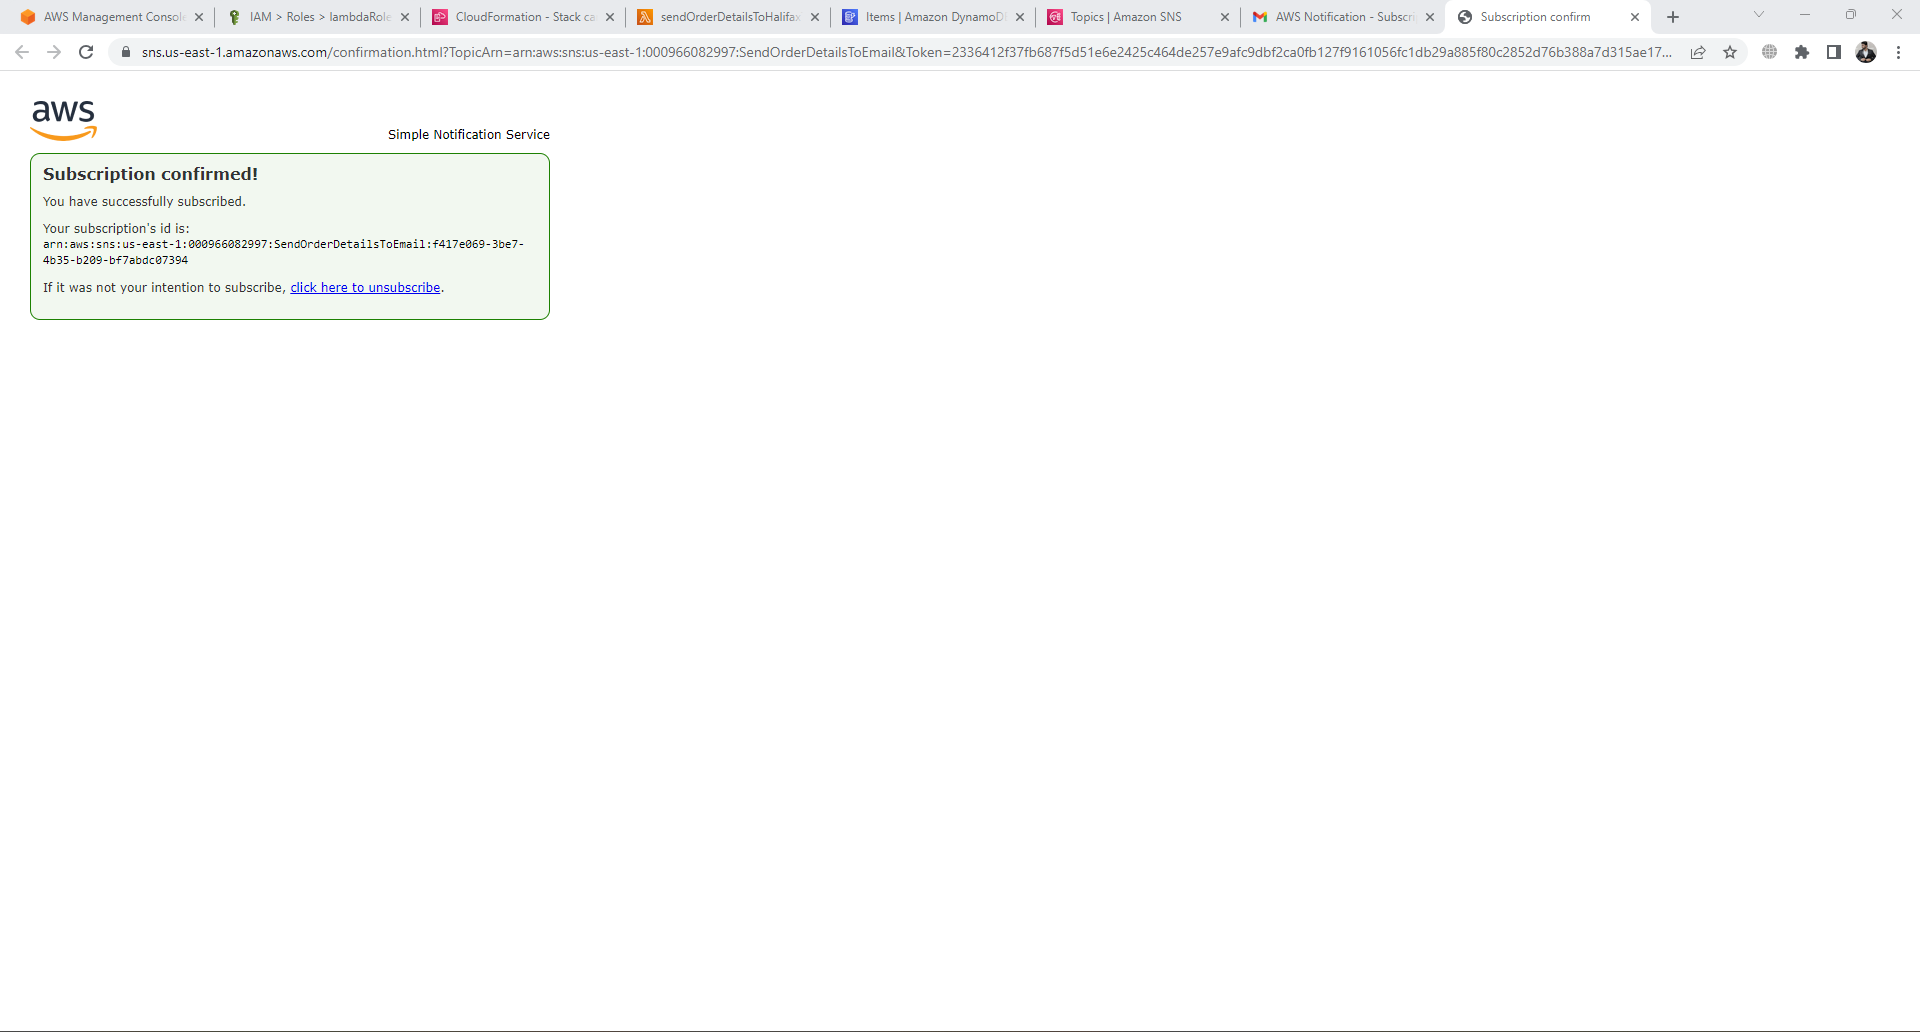
\includegraphics[scale=1, width=15cm]{PROBLEM 3/Screenshots/2.4 confirmed subscription.png}
        \caption{\textbf{\textit{Confirmed subscription}}}
        \label{fig:}
    \end{figure}

    \begin{figure}[htp]
        \centering
        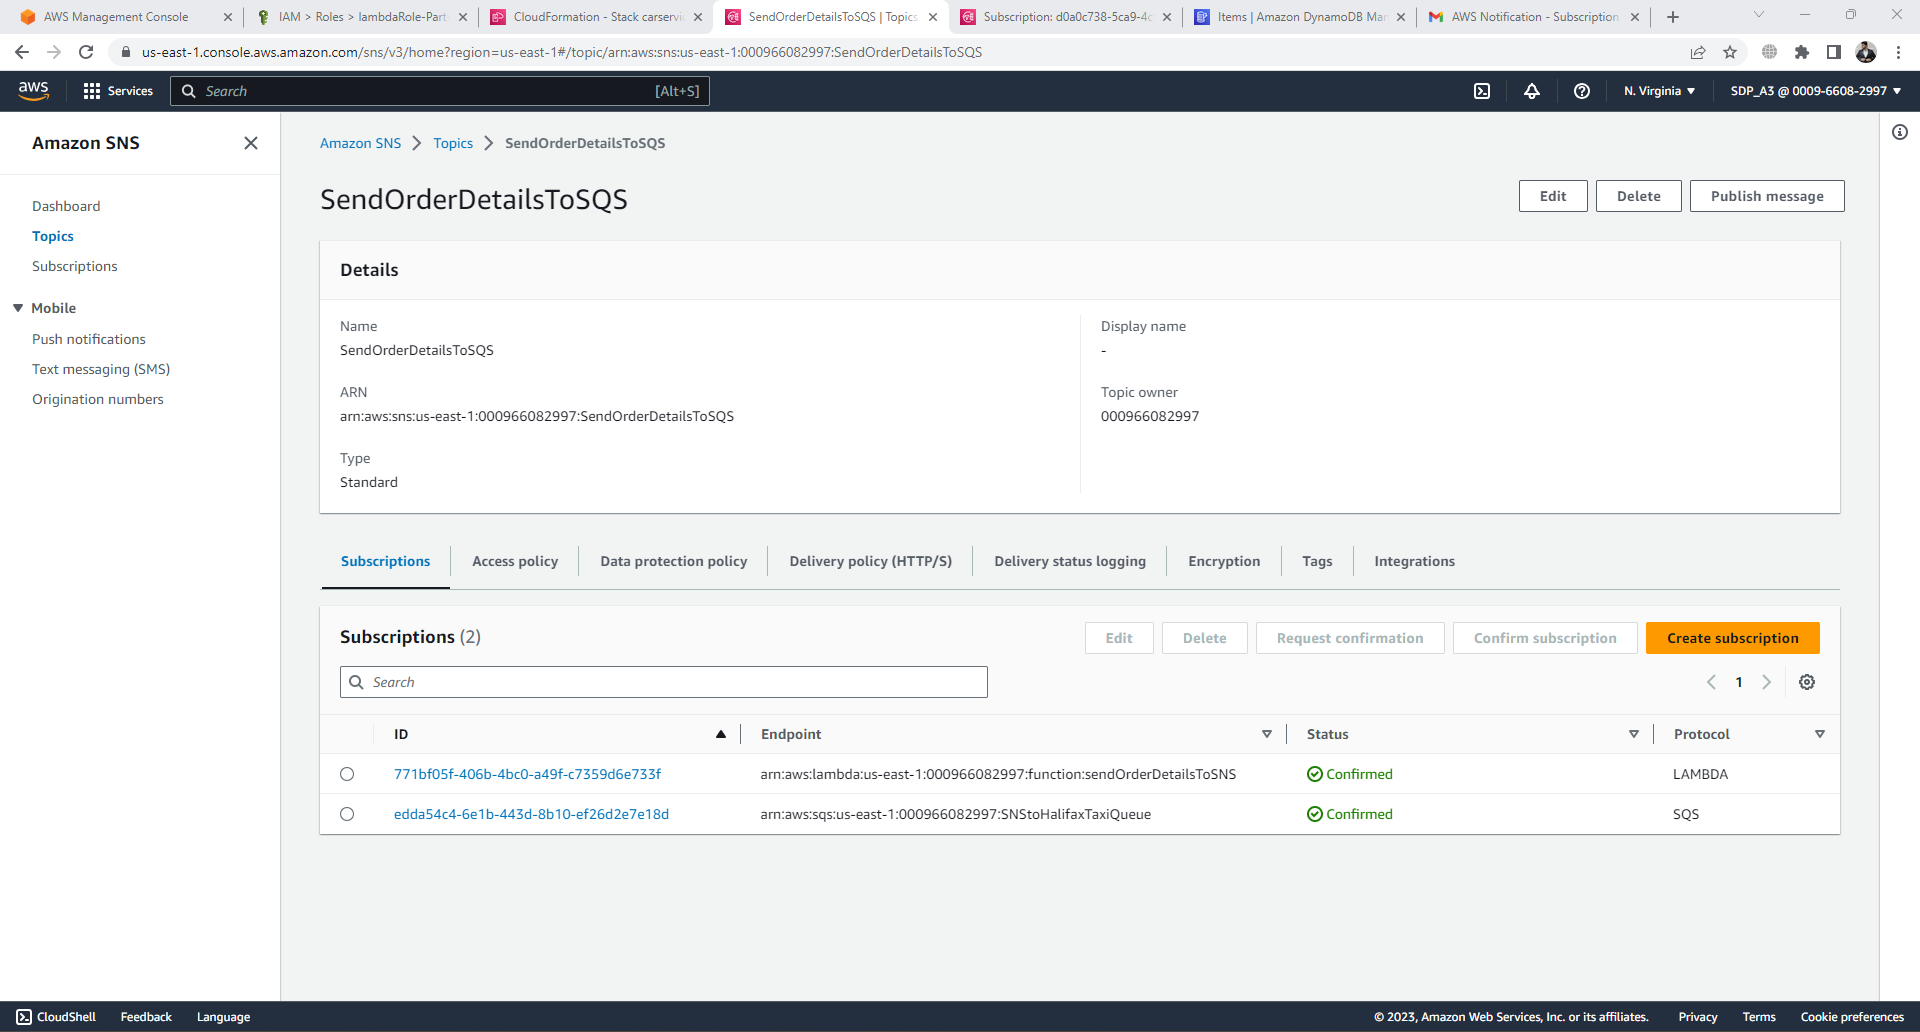
\includegraphics[scale=1, width=15cm]{PROBLEM 3/Screenshots/3.1 subscriptions of topic=SendOrderDetailsToSQS.png}
        \caption{\textbf{\textit{Subscriptions of topic=SendOrderDetailsToSQS}}}
        \label{fig:}
    \end{figure}

    \begin{figure}[htp]
        \centering
        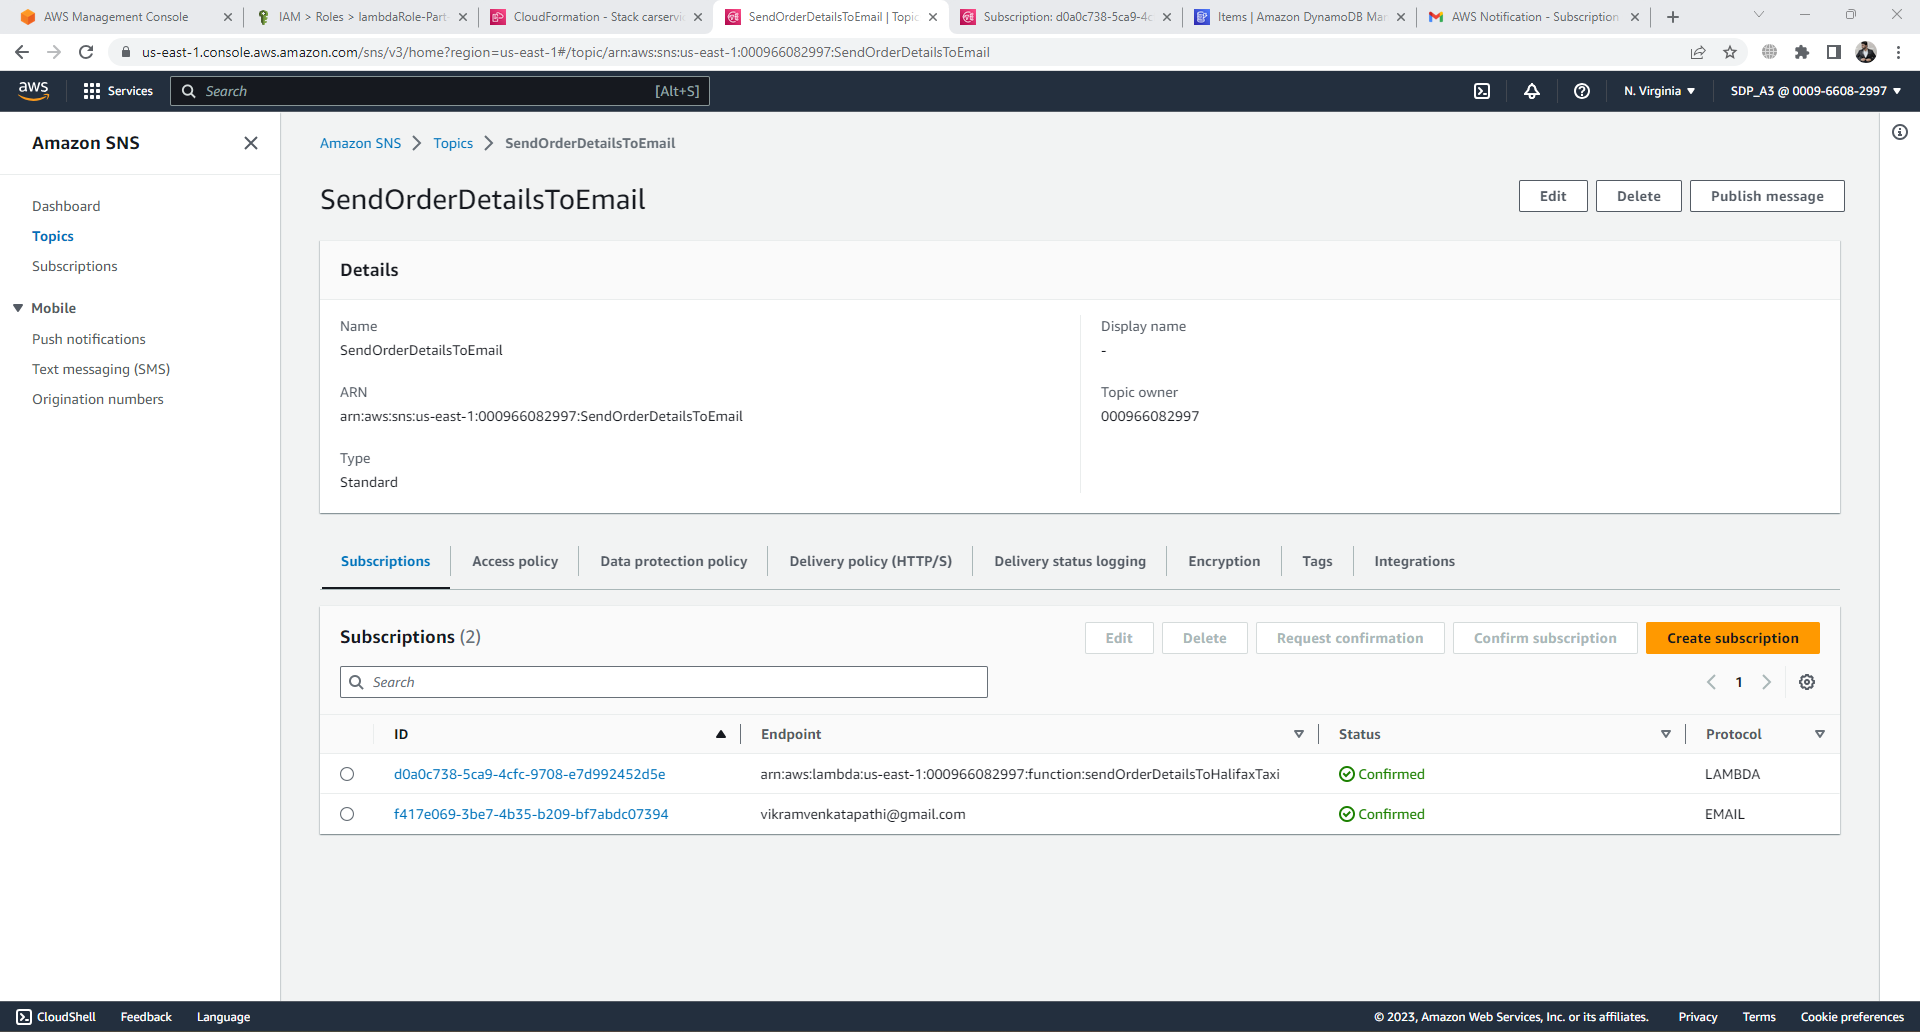
\includegraphics[scale=1, width=15cm]{PROBLEM 3/Screenshots/3.2 subscriptions of topic=SendOrderDetailsToEmail.png}
        \caption{\textbf{\textit{Subscriptions of topic=SendOrderDetailsToEmail}}}
        \label{fig:}
    \end{figure}

    \begin{figure}[htp]
        \centering
        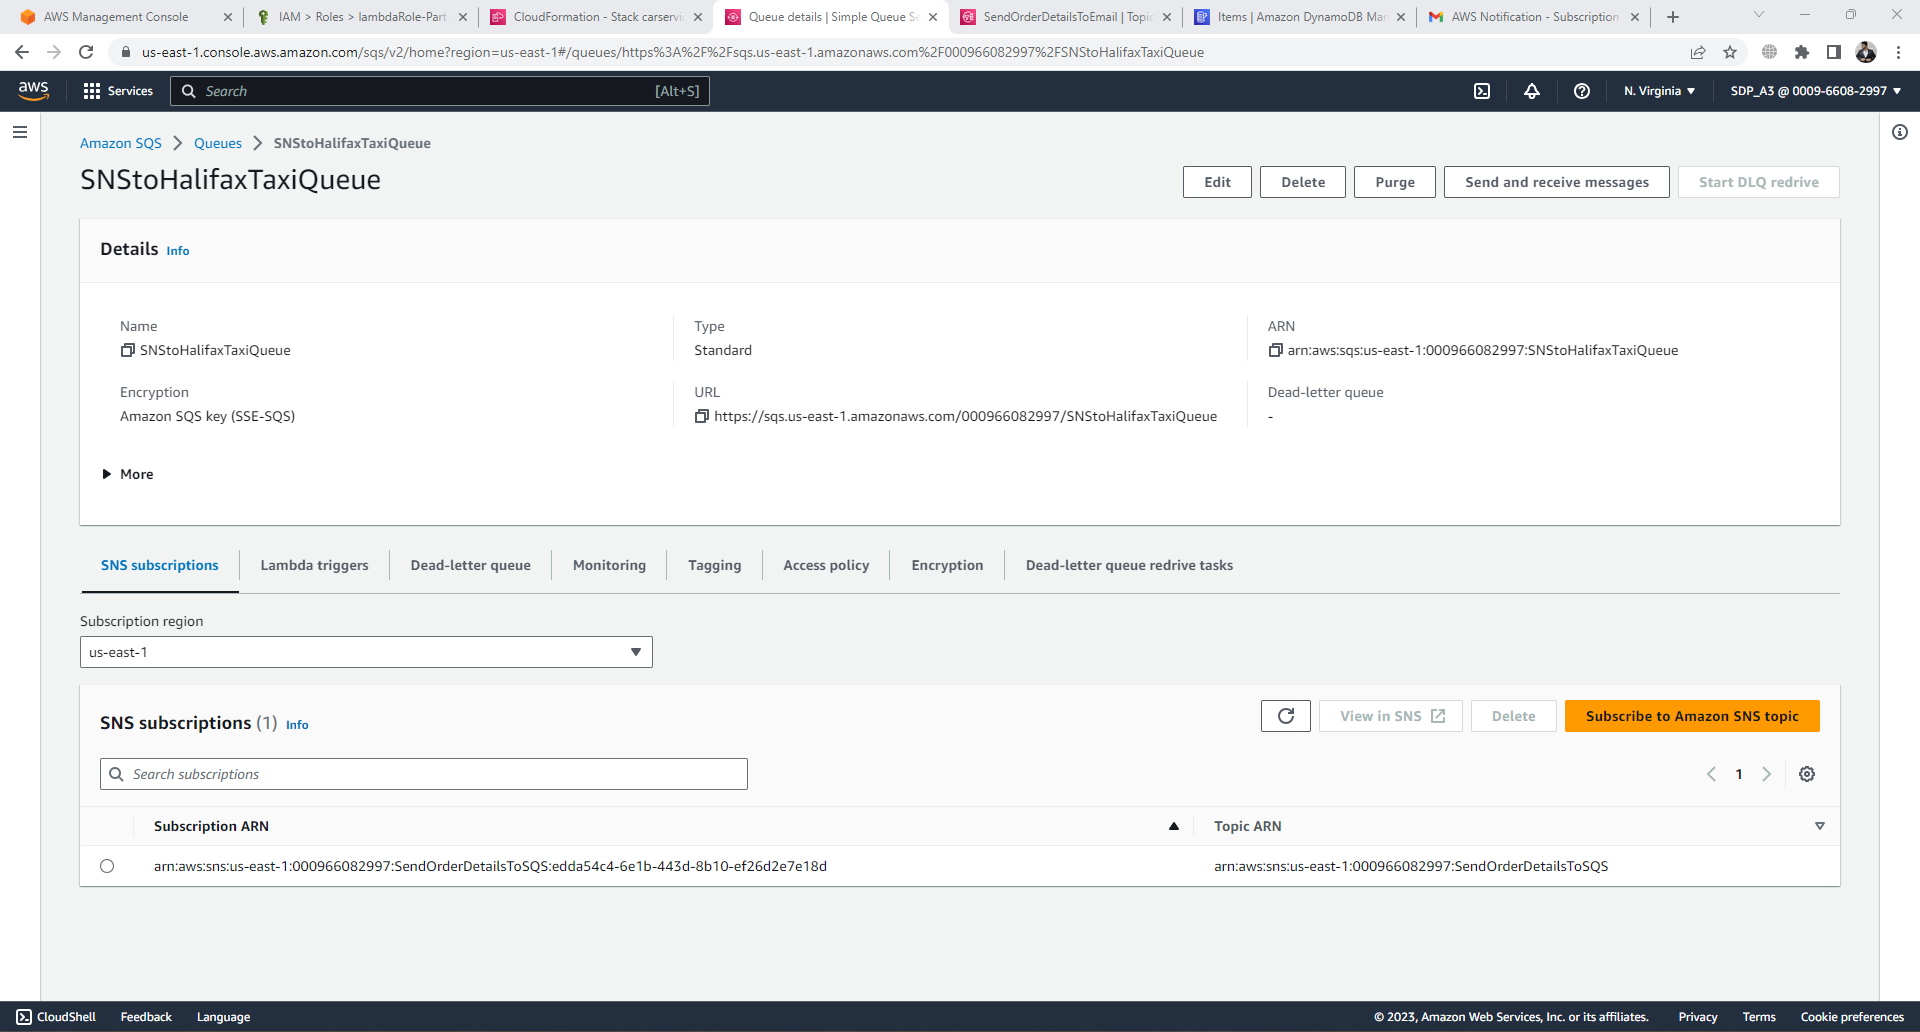
\includegraphics[scale=1, width=15cm]{PROBLEM 3/Screenshots/3.3 SNStoHalifaxTaxiQueue - SNS subscriptions.png}
        \caption{\textbf{\textit{SNStoHalifaxTaxiQueue - SNS subscription}}}
        \label{fig:}
    \end{figure}

    \begin{figure}[htp]
        \centering
        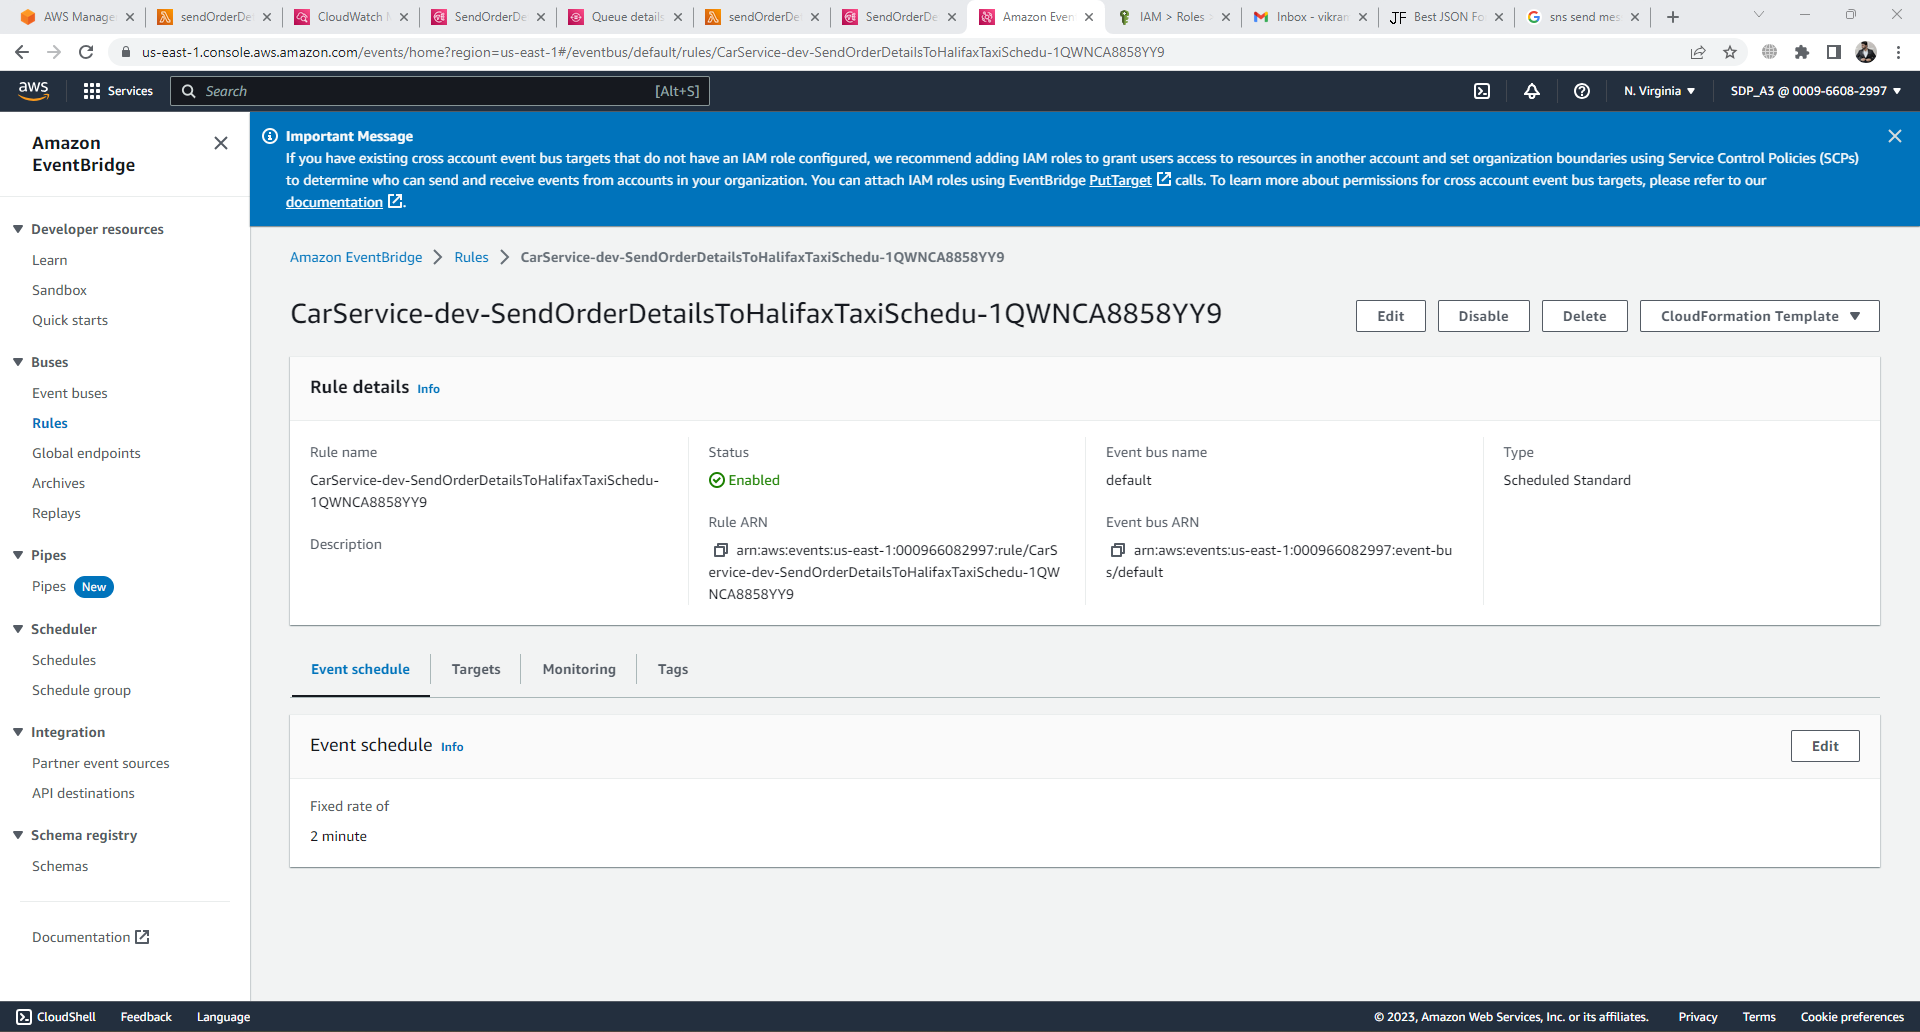
\includegraphics[scale=1, width=15cm]{PROBLEM 3/Screenshots/3.4 Event rule created for SendOrderDetailsToHalifaxTaxiSchedu lambda.png}
        \caption{\textbf{\textit{Event rule "CarService-dev-SendOrderDetailsToHalifaxTaxiSchedu-1QWNCA8858YY9", created for Lambda: SendOrderDetailsToHalifaxTaxi }}}
        \label{fig:}
    \end{figure}

    \begin{figure}[htp]
        \centering
        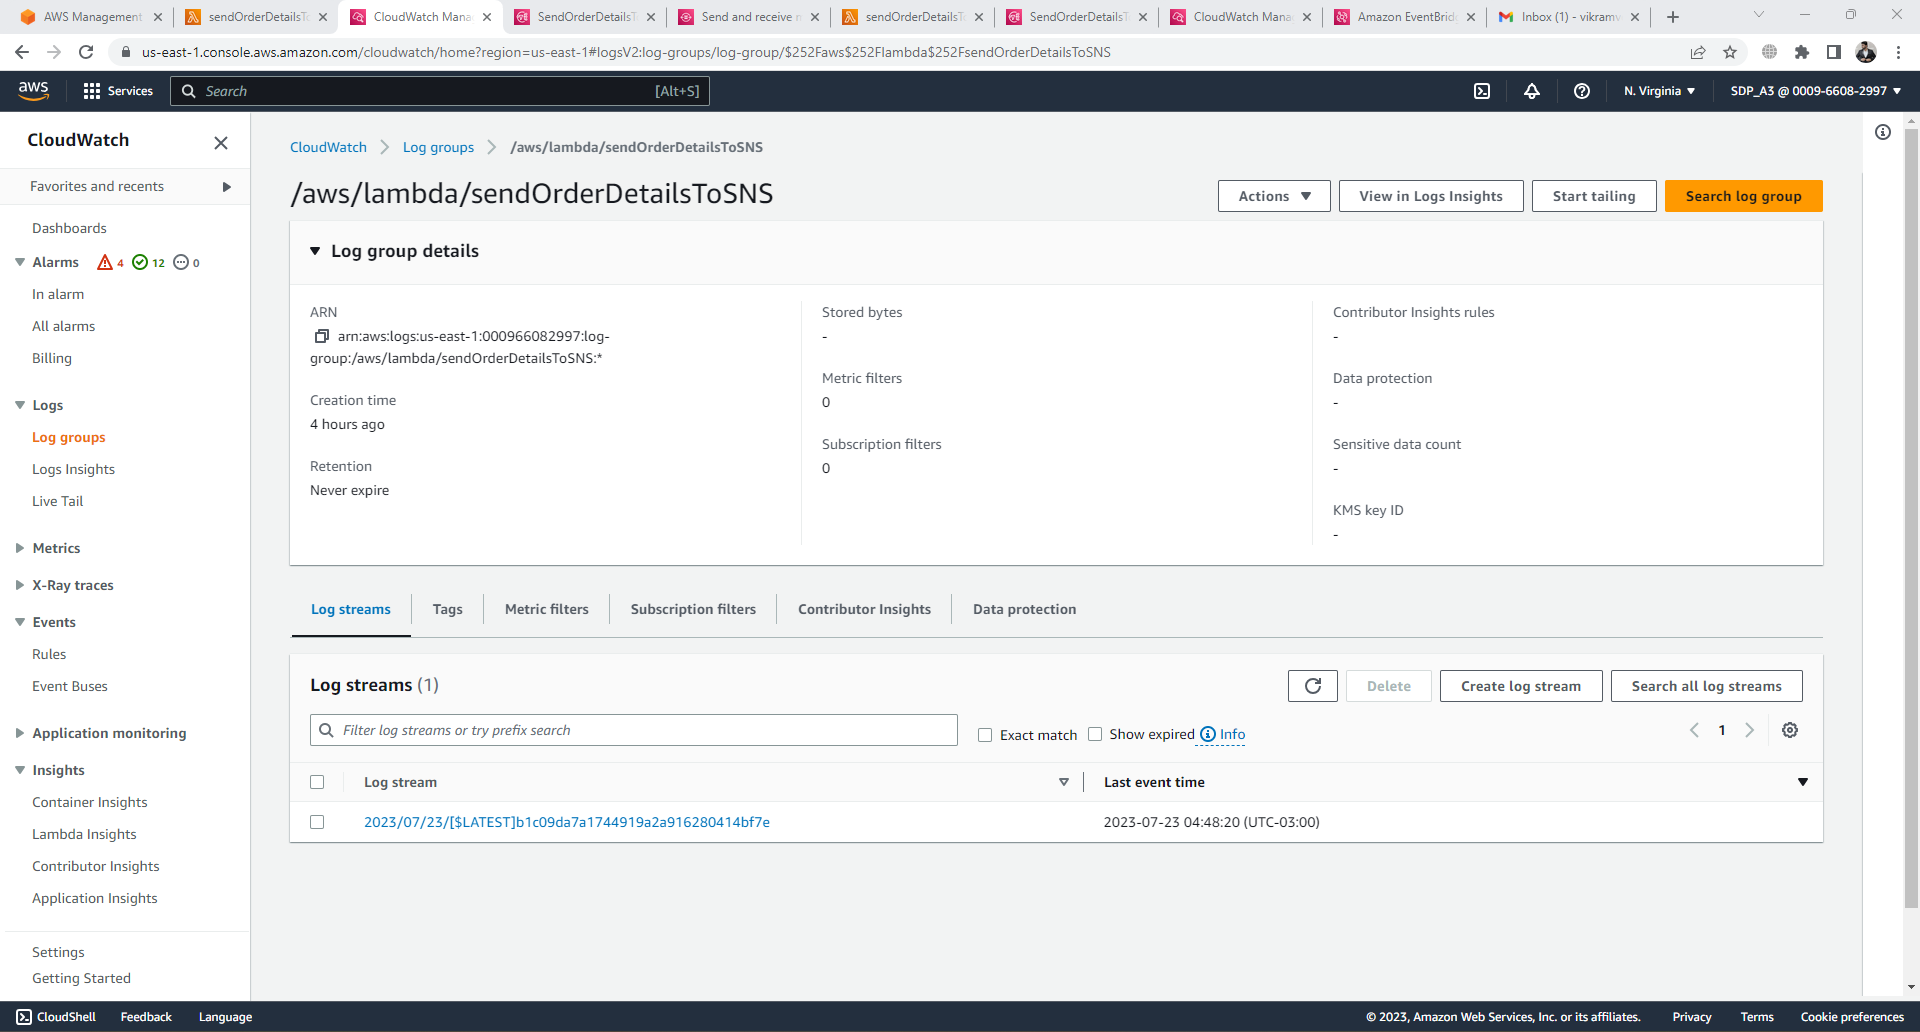
\includegraphics[scale=1, width=15cm]{PROBLEM 3/Screenshots/4.1 sendOrderDetailsToSNS lambda - send message - logs.png}
        \caption{\textbf{\textit{sendOrderDetailsToSNS lambda - send message logs}}}
        \label{fig:}
    \end{figure}

    \begin{figure}[htp]
        \centering
        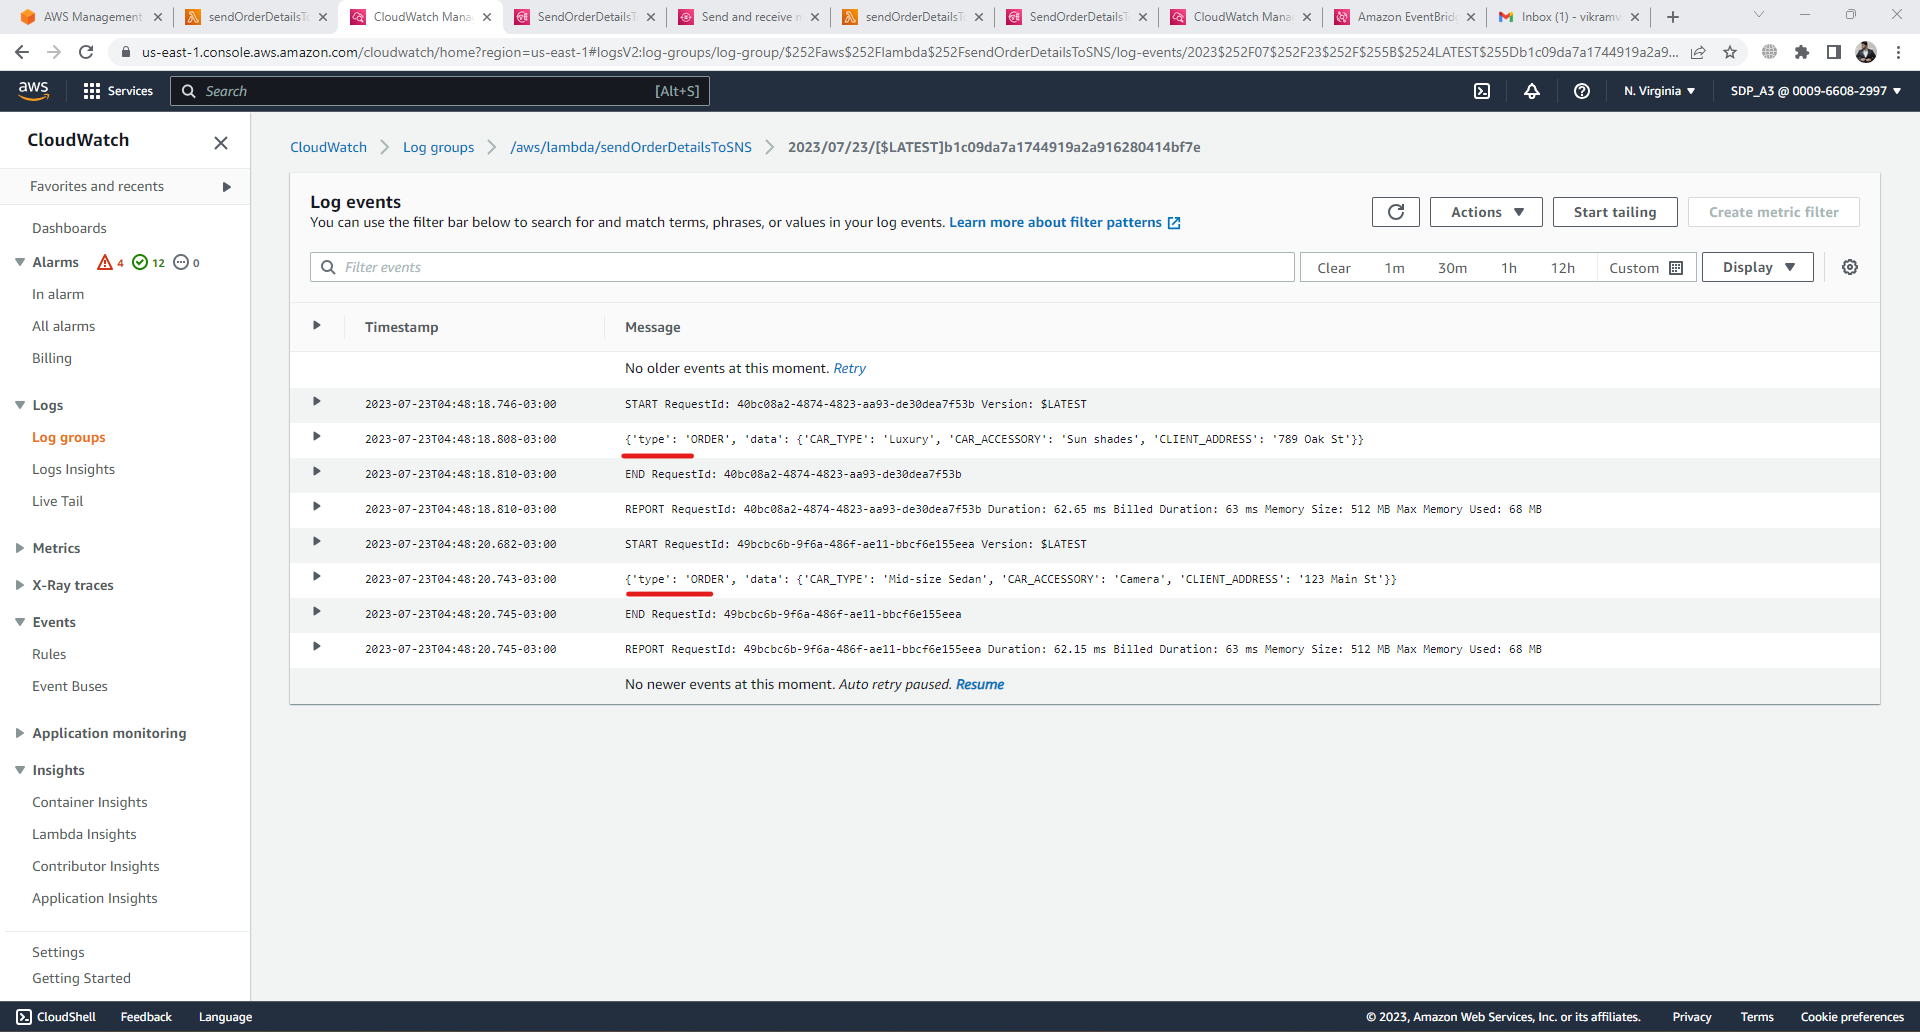
\includegraphics[scale=1, width=15cm]{PROBLEM 3/Screenshots/4.2 sendOrderDetailsToSNS lambda - send message - 2 messages sent.png}
        \caption{\textbf{\textit{sendOrderDetailsToSNS lambda - send message logs- 2 messages sent}}}
        \label{fig:}
    \end{figure}

    \begin{figure}[htp]
        \centering
        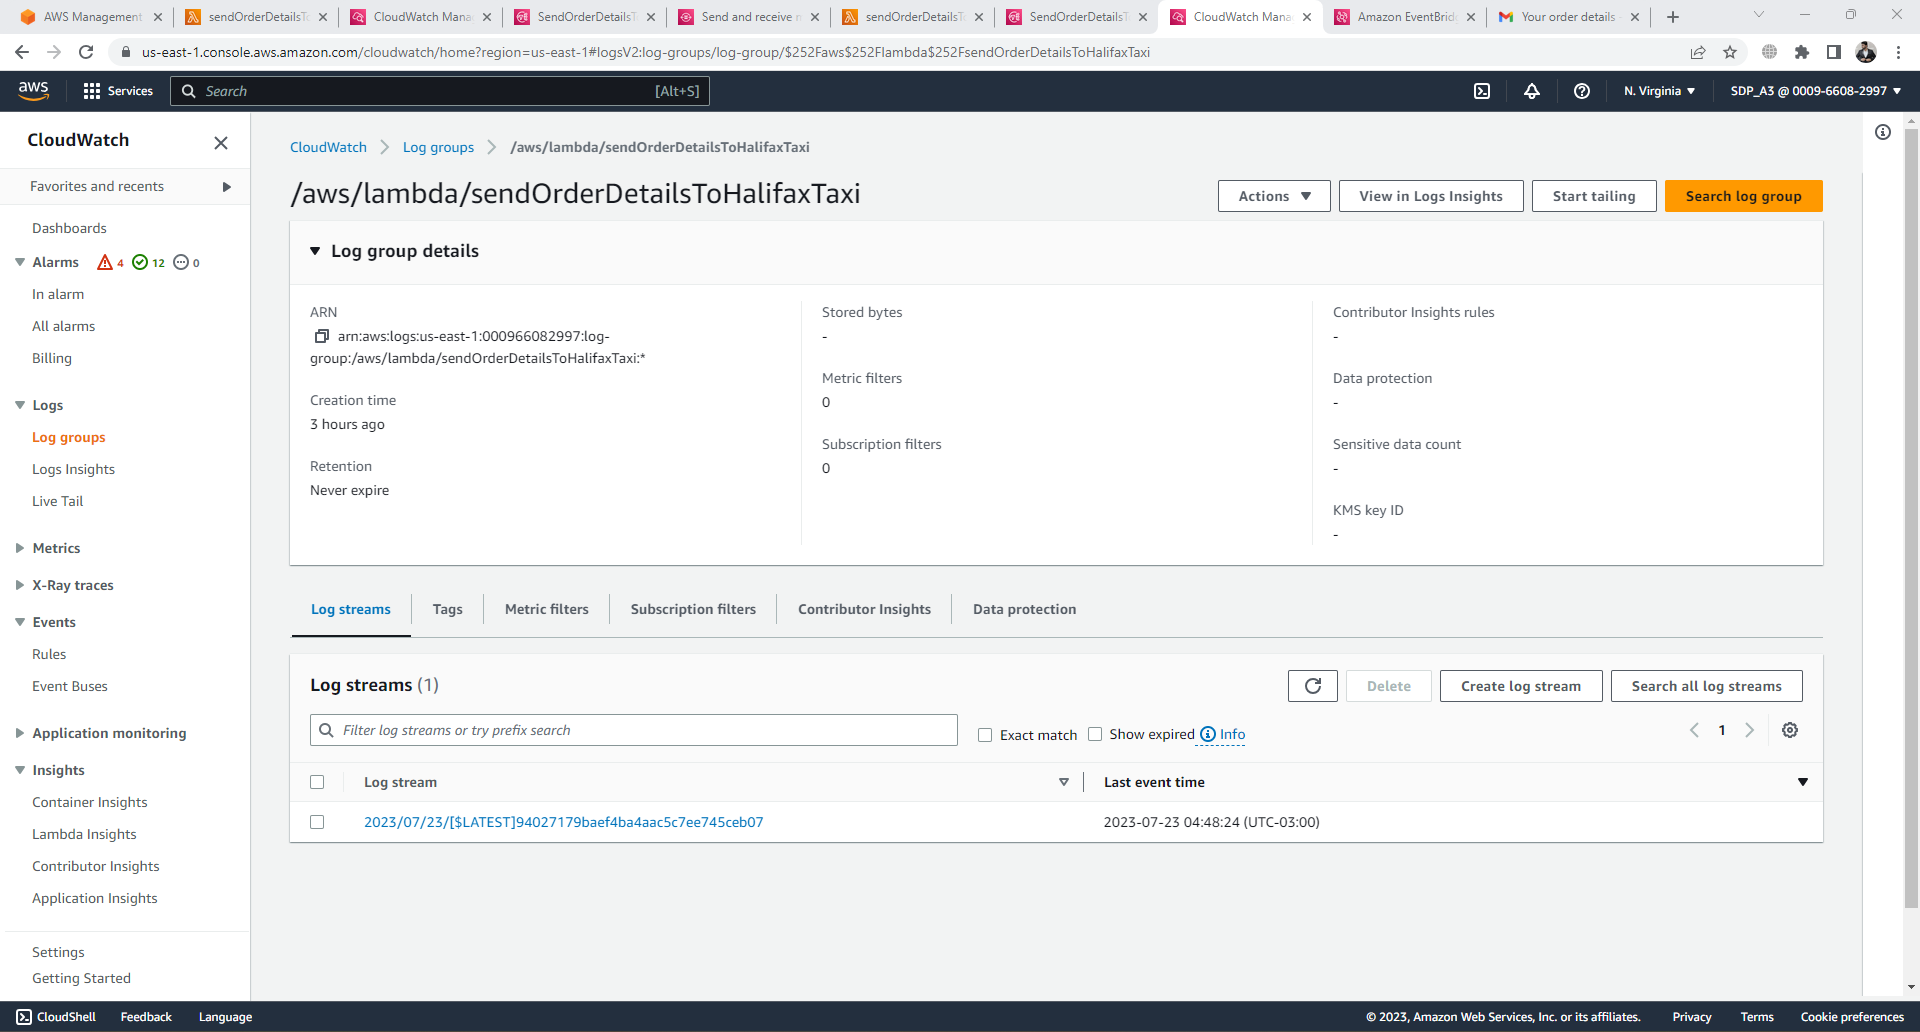
\includegraphics[scale=1, width=15cm]{PROBLEM 3/Screenshots/5.1 sendOrderDetailsToHalifaxTaxi lambda - receive msgs - logs.png}
        \caption{\textbf{\textit{sendOrderDetailsToHalifaxTaxi lambda - receive msgs logs}}}
        \label{fig:}
    \end{figure}

    \begin{figure}[htp]
        \centering
        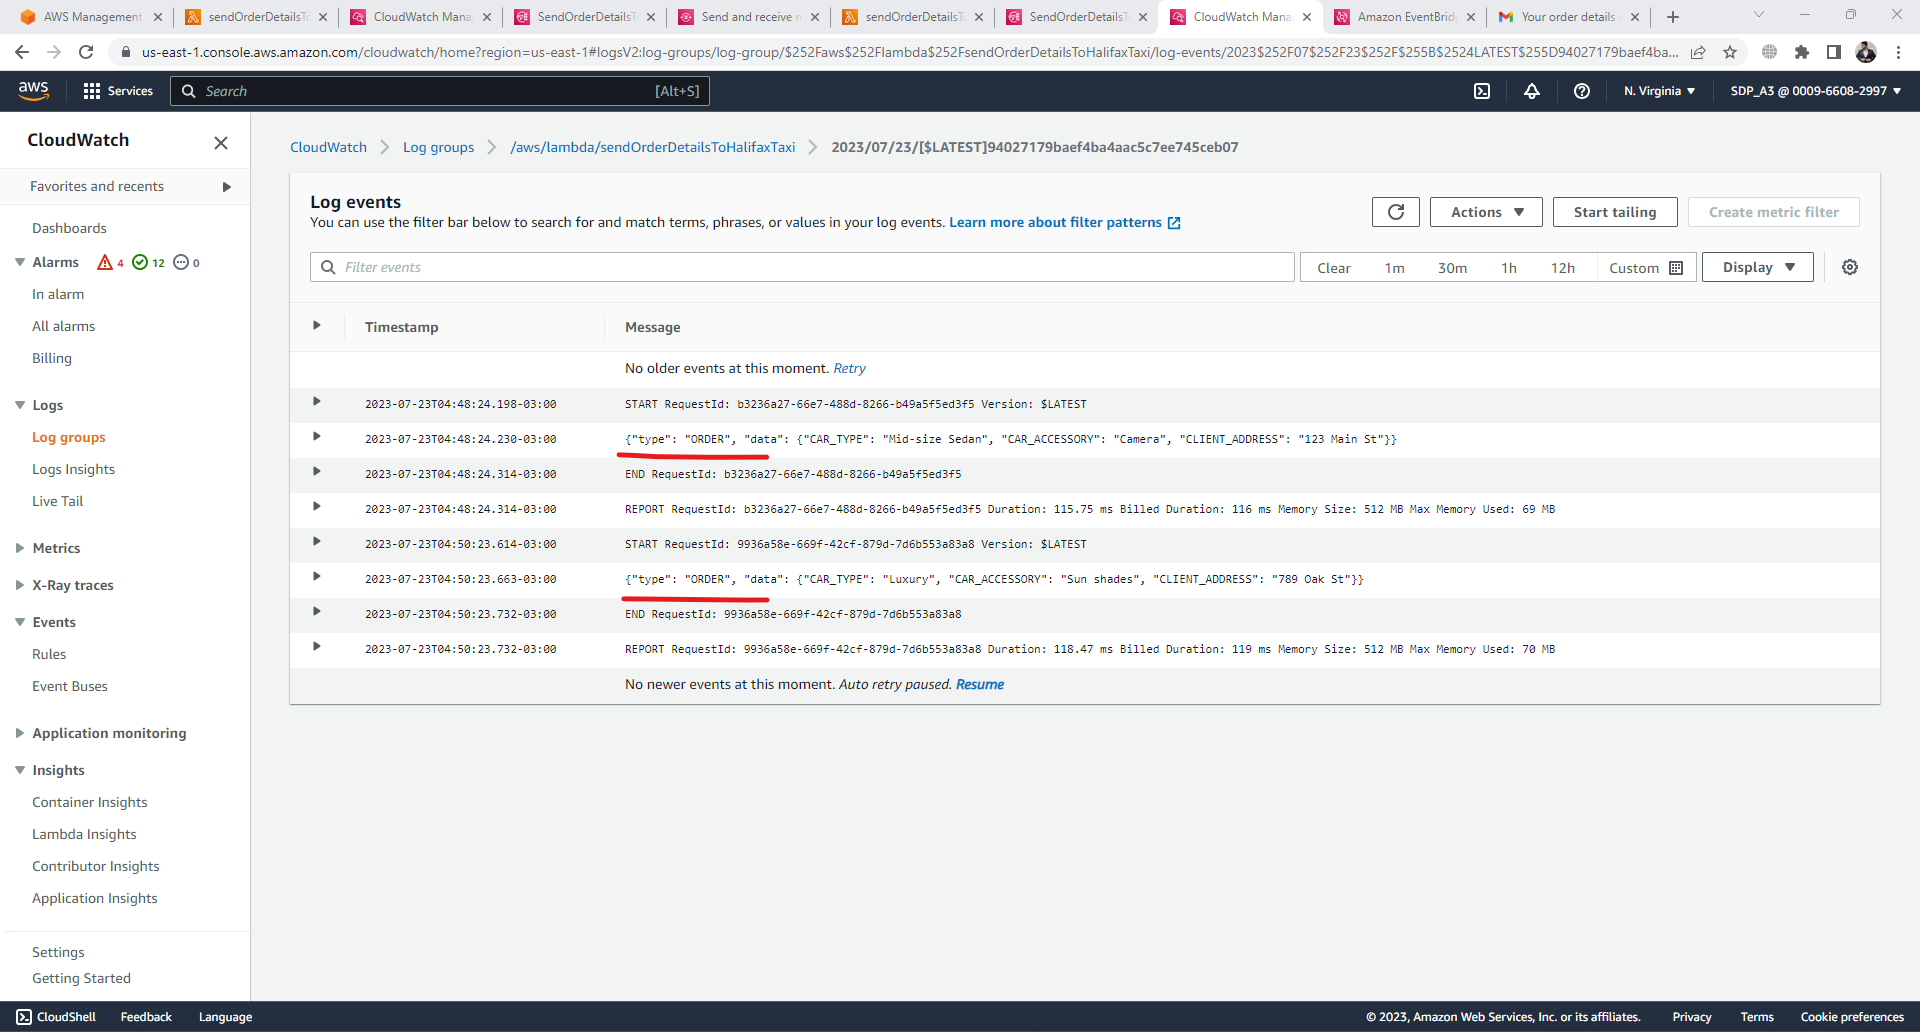
\includegraphics[scale=1, width=15cm]{PROBLEM 3/Screenshots/5.2 sendOrderDetailsToHalifaxTaxi lambda - receive msgs logs - 2 msgs received.png}
        \caption{\textbf{\textit{sendOrderDetailsToHalifaxTaxi lambda - receive msgs logs - 2 msgs received}}}
        \label{fig:}
    \end{figure}

    \begin{figure}[htp]
        \centering
        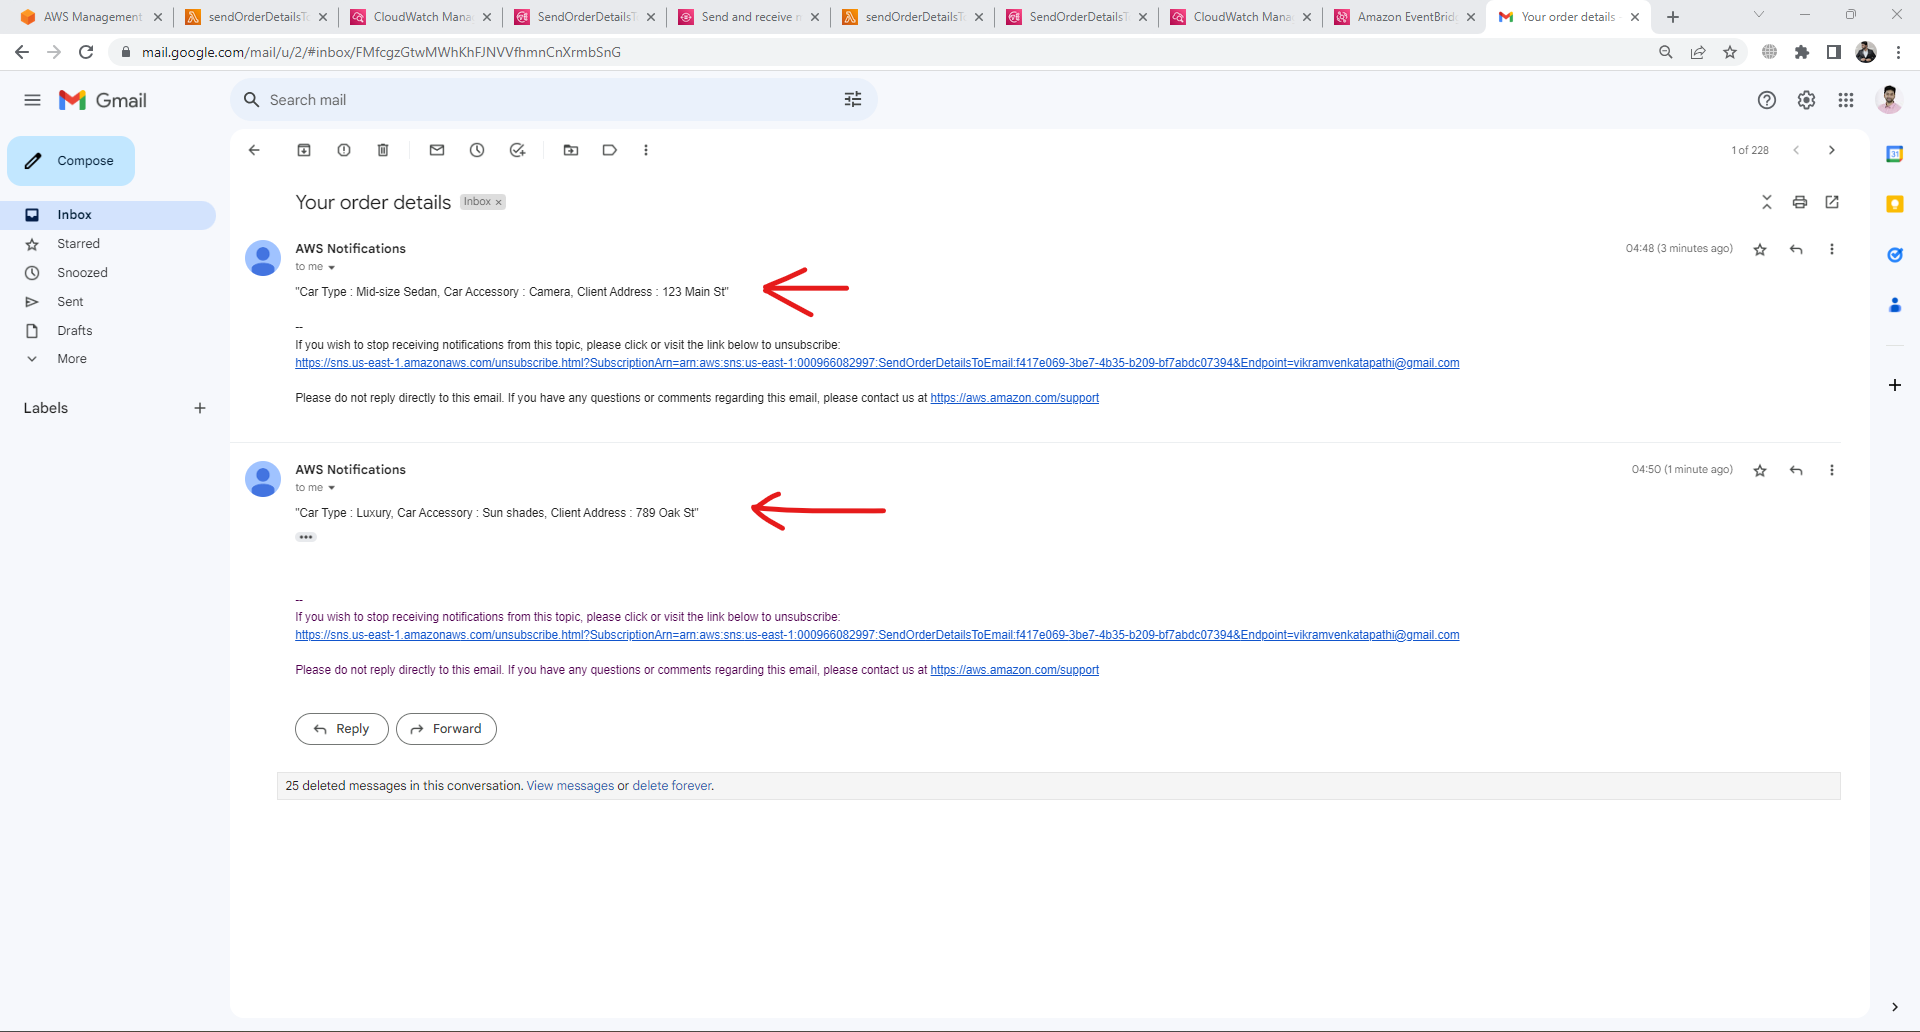
\includegraphics[scale=1, width=15cm]{PROBLEM 3/Screenshots/6.1 2 emails received.png}
        \caption{\textbf{\textit{2 Emails with order details - received}}}
        \label{fig:}
    \end{figure}

    \begin{figure}[htp]
        \centering
        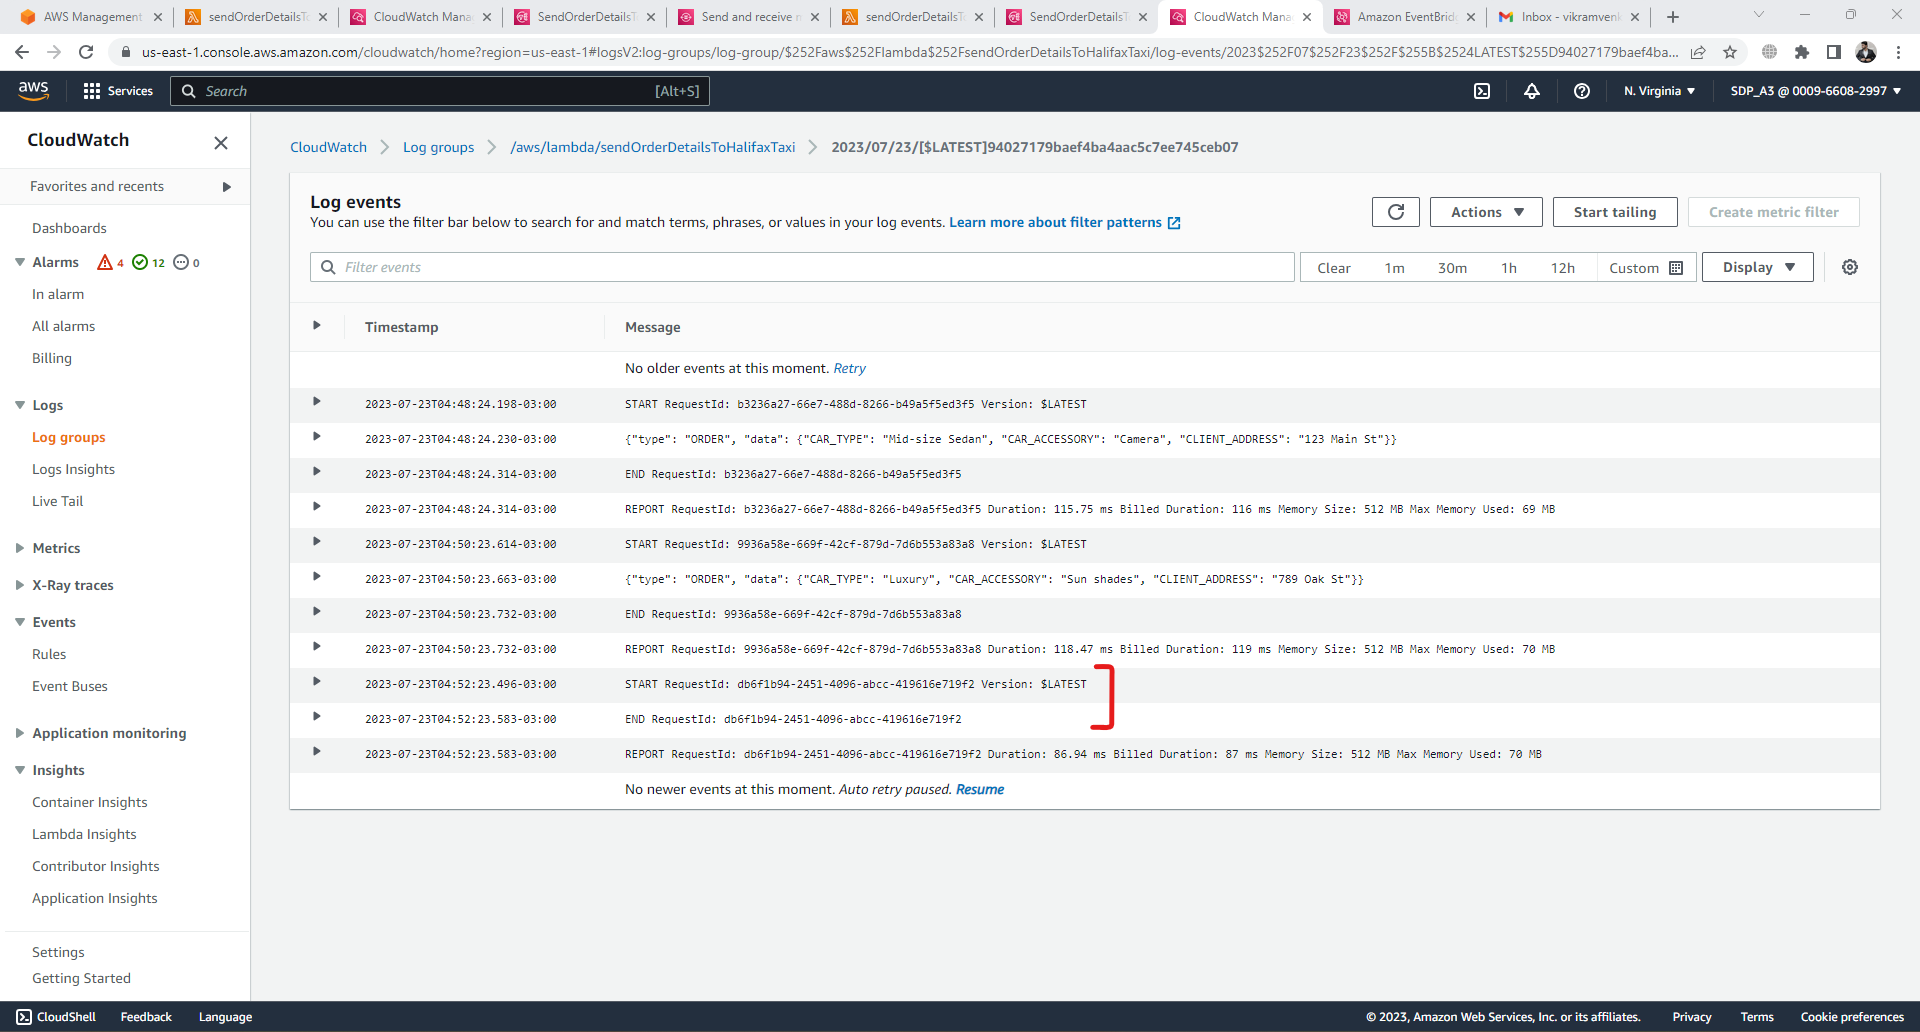
\includegraphics[scale=1, width=15cm]{PROBLEM 3/Screenshots/7.1 No more msgs in queue - so empty - didnt send any mail.png}
        \caption{\textbf{\textit{No more msgs in the queue - so empty lambda invoke- didn't send any mail }}}
        \label{fig:}
    \end{figure}
    
    
    % \begin{figure}[htp]
    %     \centering
    %     \includegraphics[scale=1, width=15cm]{PROBLEM 3/Screenshots/}
    %     \caption{\textbf{\textit{}}}
    %     \label{fig:}
    % \end{figure}
    
